\documentclass[a4paper, 11pt, twoside, openright]{book}

% \usepackage[utf8]{inputenc}
\usepackage{graphicx}
\usepackage{fancyhdr}
\usepackage{tabularx}
\usepackage{amsmath} % advanced math
\usepackage[hidelinks]{hyperref} % hide ugly boxes around links + add urls support
\usepackage{indentfirst} % intend first paragraph
\usepackage{algpseudocode} % add pseudocode
\usepackage{algorithm} % fancier pseudocode
\usepackage{array} % better alignments of tables
% \usepackage{emoji}
\usepackage{pdfpages} % to include pdf
\usepackage{dirtree} % directory representation

% set paths
\graphicspath{{assets/}}

% Setting penalty for breaking line or page after[before] first[last] line of
% paragraph
\clubpenalty=10000
\widowpenalty=10000

% line formatting
\linespread{1.1}

% this fixes warning during compilation and makes head bigger
\setlength{\headheight}{13.6pt}

% Bibliography setting
% \usepackage[backend=biber, style=numeric, sorting=nty]{biblatex}
\usepackage{biblatex}
\addbibresource{biblio.bib}

% turn off page numbering for this part
\pagenumbering{gobble}

% makes sure that the page is on the left
\makeatletter
\newcommand*{\cleartoleftpage}{%
  \clearpage
    \if@twoside
    \ifodd\c@page
      \hbox{}\newpage
      \if@twocolumn
        \hbox{}\newpage
      \fi
    \fi
  \fi
}
\makeatother

\begin{document}
%% initial pages


\begin{titlepage}
    \begin{center}
        
        \LARGE
        Czech Technical University in Prague\\
        Faculty of Electrical Engineering\\
        Department of Computer Science
        
        
\includegraphics[width=0.4\textwidth]{assets/ctu_blackwhite.jpg}

        \Large
        \textbf{Diploma Thesis}
        
        \vfill
        
        \vspace*{0.5cm}
        \LARGE
        % \textbf{Fides: A Trust Model for Collaborative Defense in Highly Adversarial Networks}
        \textbf{Trust Model for Global Peer-To-Peer Intrusion Prevention System} 
        
        \vfill

        \large
        Author: Bc. Lukáš Forst \\
        Supervised by Garcia Sebastian, Assist. Prof., PhD
        
        \vspace{0.8cm}

        \Large
        May 2022

    \end{center}
\end{titlepage}

\thispagestyle{empty}
\cleardoublepage
% Assignment
% we have two pages so we want to have it together
\cleartoleftpage
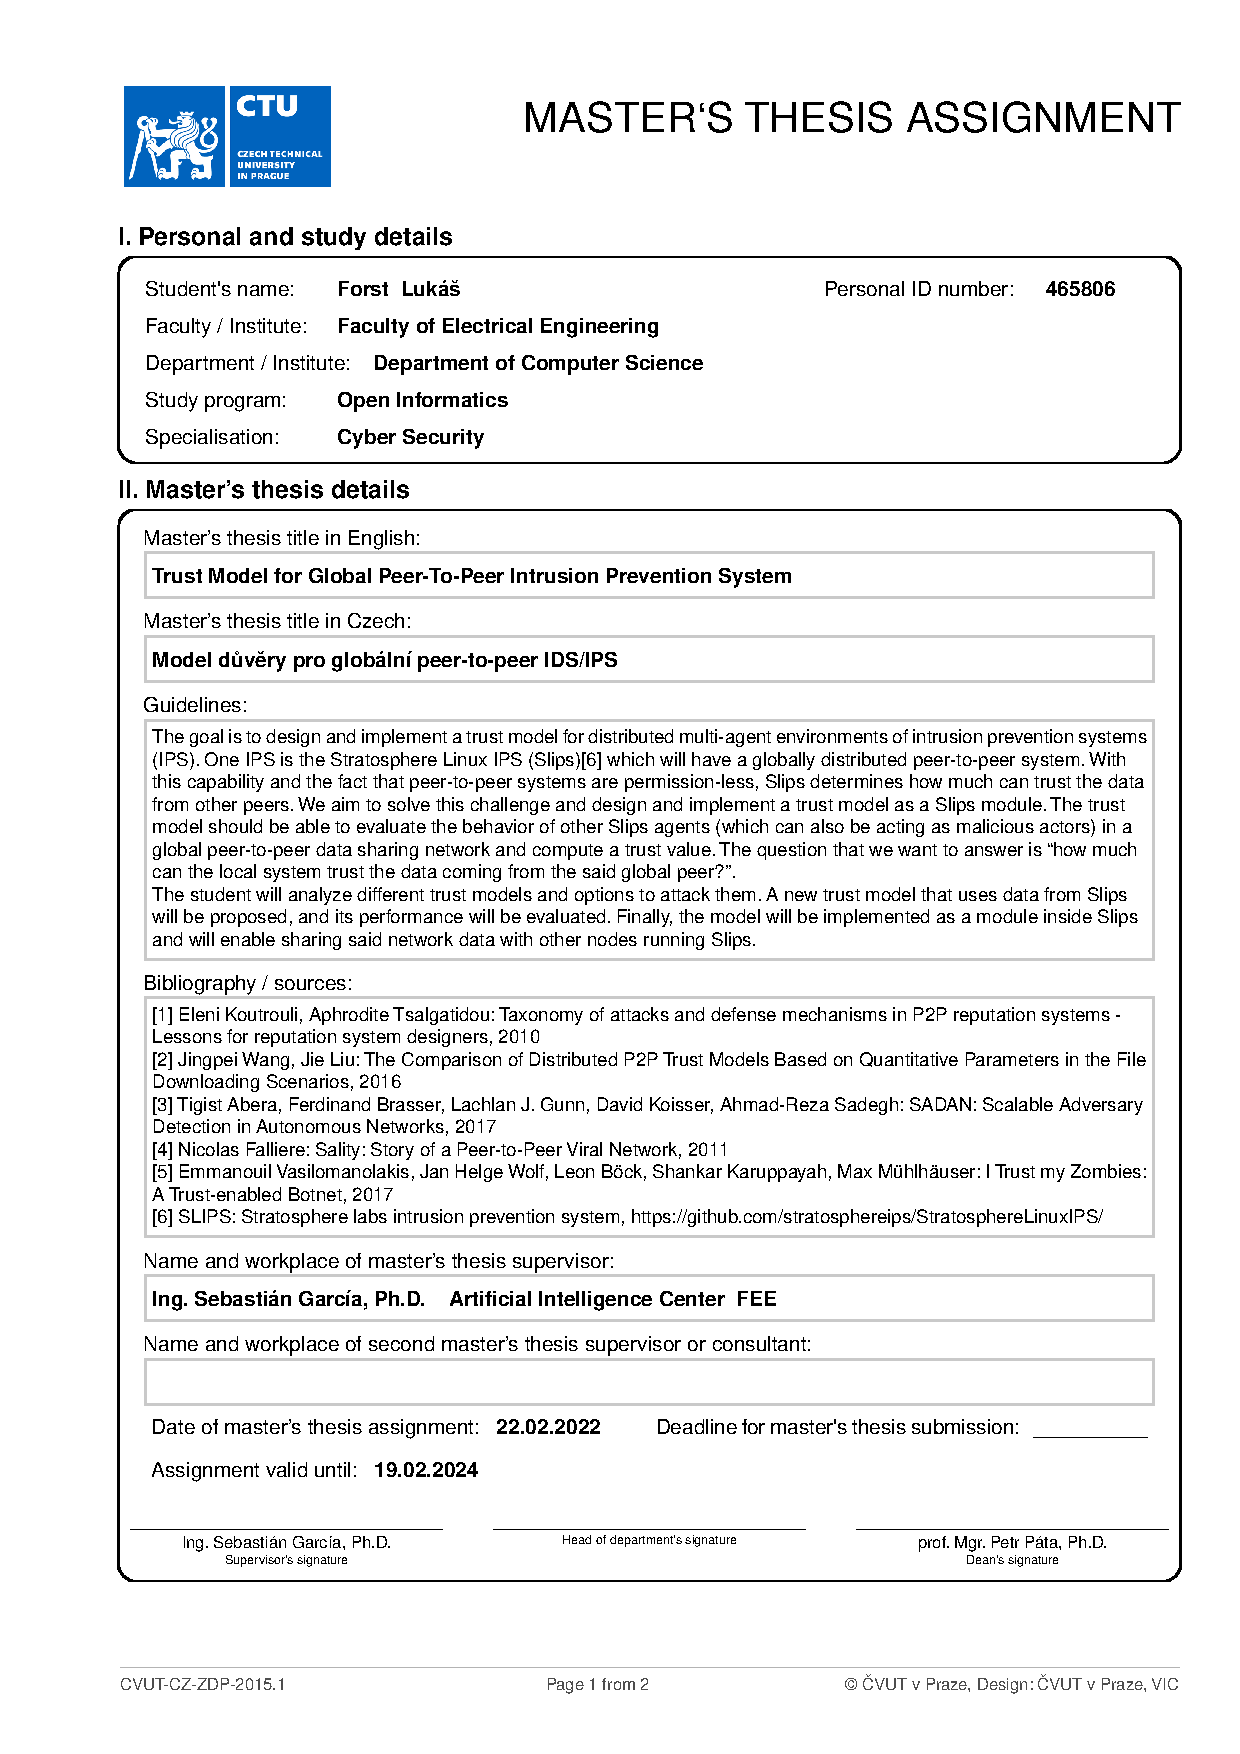
\includepdf[pages=-,scale=.8]{assets/assignment.pdf}

\section*{Declaration}
I hereby declare that the presented work has been composed solely by myself and that I have listed all sources of information used within it in accordance with the methodical instructions about ethical principles in the preparation of academic theses.

\vspace{15mm}

\begin{table}[h!]
    \centering
    \begin{tabular*}{\textwidth}{c @{\extracolsep{\fill}} c}
    \cline{1-1} \cline{2-2}
    \textit{Prague, Date}\,\,\,  & \quad\textit{Signature} \\ 
    \end{tabular*}
\end{table}

\thispagestyle{empty}

\cleardoublepage
\vspace*{\fill}

\section*{Acknowledgment}
First and foremost, I would like to thank my supervisor Sebastian Garcia for countless consultations and brainstormings and mainly for the significant amount of his time he invested in me and this thesis. Thank you.

I want to say thank you to the whole Stratosphere Research Laboratory, specifically to Veronica Valeros, Maria Rigaki, and Ondřej Lukáš, for providing me with all support I needed, for proofreading the thesis, and for guiding me through the academic world.
I'm grateful for doing this work with you and being part of the team in Stratosphere.

Finally, I must express my very profound gratitude to my parents and my whole family for providing me with unfailing support and continuous encouragement throughout my years of study and through the process of researching and writing this thesis. 

\bigskip \noindent
This accomplishment would not have been possible without you.
  
\bigskip \noindent
Thank you.
  
\bigskip \noindent
\hspace*{0.6\textwidth} 
\includegraphics[width=0.4\textwidth]{assets/signature.png}

\thispagestyle{empty}

\cleardoublepage
\newenvironment{abstractpage}
  {\cleardoublepage\thispagestyle{empty}}
  {\vfill\cleardoublepage}
\newenvironment{abstract}[1]
  {\bigskip
   \begin{center}\bfseries#1\end{center}\small\leftskip=0.5cm\rightskip=0.5cm}
  {\par\bigskip}

\providecommand{\keywords}[2]{\footnotesize\textbf{\textit{#1:}} #2}

\begin{abstractpage}
\begin{abstract}{Abstract}

Most network defense systems only rely on evidence-based knowledge about past cyberattacks, known as threat intelligence. Firewalls and intrusion prevention systems rely on the shared threat intelligence generated by other systems to prevent attacks before is too late.
Such threat intelligence is usually shared via centralized public and private blocklists where a single centralized authority, hopefully, has complete control over what is published. Such centralized system has many issues: single point of failure both technically and in trust, lack of flexibility on new data and providers, and manual trust in the providers.

To mitigate these problems, peer-to-peer networks can be used to share threat intelligence. However, because these networks are open to anyone, including malicious actors, the peers need to be able to determine who to trust and which data is better to discard.

This thesis introduces Fides. Fides is a generic trust model fine-tuned for sharing security threat intelligence in highly adversarial global peer-to-peer networks of intrusion prevention agents.
We design and built Fides taking into account the problems and limitations of previous state-of-the-art trust models, optimizing it for a broad spectrum of peer-to-peer networks where peers can join and leave at any time.
Fides evaluates the behavior of peers in the network, including their membership in pre-trusted organizations and uses this knowledge to compute the trust.
Fides continually assesses received data from the peers and by weighting and comparing them with each other is able to determine which peer provides better services. The received threat intelligence is always aggregated and weighted and then provided to the underlying intrusion prevention system.
Among many results, our experiments show that if at least 25\% of peers are part of trusted organizations, then 75\% of the network can be \textit{completely controlled by the malicious actors}, and Fides would still be able to provide the correct values of the threat intelligence data to the peers. We conclude that Fides is a suitable solution for modeling trust in global adversarial peer-to-peer networks. 

The direct contribution of this thesis is the computational model of the trust model Fides, the reference implementation of the model in Python, the simulation framework for modeling peers' behavior in the network including the implementation of the framework and the implementation of the Fides module for reference intrusion prevention system.

\end{abstract}

\keywords{Keywords}{trust models, threat intelligence, collaborative network defense, intelligence sharing}

\vspace*{\fill}

\newpage
\begin{abstract}{Abstrakt}
    TBD \todo{add cz absrakt}
    
\end{abstract}
\keywords{Klíčová slova}{TBD1, TBD2} \todo{add cz kws}

\end{abstractpage}
\thispagestyle{empty}

\cleardoublepage

% first start roman page numbering
\pagestyle{plain}
\frontmatter 

% table of contents 
\tableofcontents
\cleardoublepage

% list of figures
%  TODO: enable this if necessary
\begingroup
\let\cleardoublepage\relax
\listoffigures
\clearpage
\endgroup

% % list of tables
\begingroup
\let\clearpage\relax
\let\cleardoublepage\relax
\listoftables
\endgroup
\cleardoublepage

 % From now on Arabic page numbering
\mainmatter

% Set header and footer styles
\pagestyle{fancy}
\fancyhf{}
\fancyhead[LE,RO]{\leftmark}
\fancyfoot[CE,CO]{\thepage}


\chapter{Conclusion}
\label{ch:conclusion}

In this thesis, we proposed, designed, and implemented \textbf{Fides}. Fides is a generic trust model fine-tuned for sharing security threat intelligence in highly adversarial global peer-to-peer networks of intrusion prevention agents.
Fides enables threat intelligence sharing in global peer-to-peer networks of Intrusion Prevention Agents agents and allows them to cooperate against malicious actors without compromising the security of the local environment. 
Although Fides is fine-tuned for threat intelligence sharing, it is generic and can be easily modified to share any other IoC data.

Fides can recognize that peers belong to different organizations. If the administrator trusts them, Fides can use this knowledge to provide better results and be more confident in its decisions.
Thanks to its granular configuration, Fides allows the administrator to set up intelligence sharing between specific organizations or share specific data only with highly trusted peers.
This ensures that Fides shares only data that can be shared and does not leak any sensitive information about the infrastructure it runs in.

The trust model itself is generic and can be integrated into any modular intrusion detection or prevention system. We chose to implement an integration with Slips~\cite{slips}, and as part of our work, we developed a Slips module that uses Fides for sharing and aggregating threat intelligence.
The entire trust model and the Slips module are open-source and available as free software~\cite{fidesGithub}.

In this thesis, we explore topics related to intrusion prevention systems~(\ref{sec:intrusion-detection-prevention-system}), threat intelligence~(\ref{sec:threat-intelligence}), and peer-to-peer networks~(\ref{sec:peer-to-peer-networks}) alongside with the state of the art in managing trust relationships with trust models~(\ref{sec:trust-in-p2p}) in Chapter~\ref{ch:previous-work-background}.
We conclude that we need a solution that is flexible enough to allow us to share sensitive threat intelligence in highly adversarial peer-to-peer networks.

In the following Chapter~\ref{ch:trust-model-design} we propose the trust model Fides and provide a high-level overview of its life cycle and the foundation of its calculations~(\ref{sec:general-overview-of-fides}).
The following sections discuss the problems that trust models face in peer-to-peer networks in general~(\ref{sec:cold-start-problem}).
After that, we analyze common attack vectors on the trust models~(\ref{sec:attack-vectors}) and outline the taxonomy of possible attacks on Fides~(\ref{sec:taxonomy-of-attacks}).
Once we outline all necessary preconditions, we deep dive into a computational model of Fides~(\ref{sec:computational-model}), including multiple options for evaluating interactions between the peers~(\ref{sec:interaction-evaluation-strategies}).
Because the trust model operates with threat intelligence, we propose multiple ways to aggregate network threat intelligence into a single value consumed by Slips~(\ref{sec:network-intelligence-aggregation}).

The architecture and implementation details of the trust model are then described in Chapter~\ref{ch:architecture} where we explain how Fides communicates in the network, how it can verify the data it receives, and how it ensures that no privacy-sensitive data are sent to the network.

In the next Chapter~\ref{ch:experiments}, we designed extensive test scenarios~(\ref{sec:environment-simulation}), explained how we evaluate each simulation~(\ref{sec:experiments-evaluation}), and then created and implemented an evaluation framework~(\ref{sec:simulations-execution}) that allowed us to simulate any possible setup in any possible environment.

We then evaluated the results of the experiments and the trust model in the Chapter~\ref{ch:results}, where we discovered that with a particular setup and under a condition that Fides talks to at least 25\% of pre-trusted peers, it could eventually identify targets correctly no matter how the rest of the peers behave.

Results have shown that Fides is a viable solution that tackles the problem of trust relationships in sensitive environments for threat intelligence sharing. 
We proved that Fides performs well and thus can be used to extend the existing implementation of Slips as a new module for sharing threat intelligence in the global peer-to-peer network.

Thanks to all the configurations and optimizations that Fides brings for usage inside the organizations, we believe that Fides enables the adoption of Slips Intrusion Prevention System across a broader spectrum of organizations.
We believe that Slips, combined with Fides, will enable more possibilities for sharing threat intelligence over the internet and improve the overall security of the networks that use Slips for the defense against intruders.


\section{Future Work}
\label{sec:future-work}
Even though we achieved our goal of designing a resilient trust model for sharing threat intelligence, there are multiple areas where the model can improve either by exploring different approaches or by implementing new additions to the data flow.

Most importantly, it is clear from the evaluation of simulations in Chapter~\ref{ch:results}, that Fides performs differently with different setups under different conditions.
Even though we are able to manually pick settings that ensure the best performance, this is not a perfect solution for real-world scenarios.
For that reason, we propose to explore further the following approaches.

\subsection{Exploring Interaction Evaluation Strategies}
\label{subsec:exploring-interaction-eval-strategies}
The trust model developed in this thesis is generic and it is heavily relying on the interaction evaluation function.
This means that the performance of the trust model is as good as the evaluation function.

In this work, we explored evaluation methods that are using only data from a single time window to evaluate the interactions.
However, the local peer might store the complete interaction history with all other peers and whenever it finds out that some peer reported threat intelligence, that proved to be correct after some time, the reporter's service trust should benefit from such discovery.
Another way might be storing the whole interaction history and using machine learning techniques, to discover irregularities in provided data during all communication windows.

In other words, all interaction evaluation strategies described in Section~\ref{sec:interaction-evaluation-strategies} do not utilize the knowledge from the past, or the history of the interactions.
We believe that this is an interesting space to explore more as it might lead to better performance of Fides in real-world scenarios.

\subsection{Exploring Threat Intelligence Aggregation Methods}
\label{subsec:exploring-threat-intelligence-aggregation-methods}
No threat intelligence aggregation methods explored in this thesis, described in the Section~\ref{sec:threat-intelligence}, use any other information than ones provided by the network at a single time window.
By incorporating information from the recent history, the aggregation might improve the overall detection performed by the trust model.

Moreover, there might be better ways how to aggregate the threat intelligence, or maybe the combination of multiple approaches to one might improve the final confidence in trust model decisions.
As we saw in Chapter~\ref{ch:results}, the combination of interaction evaluation and threat intelligence aggregation influences the performance of the trust model to great extent.

\subsection{Possible Mitigation of Sybil Attack}
\label{subsec:possible-mittigation-of-sybil-attack}
When analyzing the possible attack vectors for Fides, we described the Sybil attack in Section~\ref{subsec:whitewashing-and-sybil-attack} and we stated that Fides is vulnerable to this type of attack.
However, results have shown that this is true only in cases when the attacker owns more than 75\% of the network. 
If the attacker controls 75\% of the network or less, Fides has a way how to defend itself and make the correct decisions about the threat intelligence.

There are essentially two possible ways how to mitigate this type of attack even for cases where the attacker controls more than 75\% of the network.

One option is to introduce restrictions to Fides, where it uses data at most from the 75\% of peers that are not pre-trusted, and the rest, 25\% comes from the pre-trusted peers and organizations. All other data from other peers in the network would not be considered during the threat intelligence aggregation.
That would ensure that Fides always only considers a limited amount of data so it will not be vulnerable to an attacker who controls more than 75\% of the network.

The second possible solution would be making it \textit{computationally hard} for new peers to join the peer-to-peer network or generate a new peer identity.
So the attacker would need to spend either time or computational resources when generating new peer identities.
This directly does not prevent a malicious actor to perform this type of attack, but it makes it significantly harder.
However, this mitigation would need to be implemented in Iris instead of Fides.

\subsection{Adding Threat Intelligence Challenges}
\label{subsec:adding-threat-intelligence-challenges}
Fung et al~\cite{fung2008trust} explore an interesting idea of creating initial trust in remote peers by giving them \textit{computational challenges}.
In our case, challenges might be asking the remote peer for threat intelligence about the target, that the local Slips know very well and with high confidence.
When the trust model receives a response it uses the interaction evaluation strategy described in Section~\ref{subsec:use-local-threat-to-evaluate} to evaluate the received data.
The trust model can then ask multiple times to have more interactions and thus effectively \textit{probing} the remote peer and getting an estimate about its future behavior.

By using this approach, one can either replace the recommendation system or greatly improve it in cases when the trust model does not have enough pre-trusted peers.
The disadvantage might be a higher amount of messages sent across the network when the new peer is registered by the network, which could eventually lead even to a denial of service attack on the newcomers. 

This method should be explored more in detail and as the Fides is quite flexible, it can be easily incorporated into the trust model as well.

\subsection{Threat Intelligence Sharing Motivation}
\label{subsec:threat-intelligence-sharing-motivation}
The designed peer-to-peer network for threat intelligence sharing unfortunately does not promote data sharing at all.
The peers sharing threat intelligence are not gaining any benefit other than gaining trust in the eyes of other peers.
As the gained trust brings little to no benefit by itself, there is a lack of incentive for the peers to share their threat intelligence with the network.

However, we can see data and threat intelligence filtering as one of the ways how to motivate other peers to share their threat intelligence.
As we described in Section~\ref{subsec:data-filtering}, the Fides administrator can choose what threat intelligence is shared with which peers by configuring confidentiality levels with required service trust.
Using this approach, the threat intelligence is shared only with high trusted peers.
That would result in an incentive for the peers to gain the service trust which they do by sharing their own threat intelligence with the network.

Another approach is exploring the idea of \textit{payments} for the threat intelligence where the peers use some sort of cryptocurrency to \textit{pay} for the received threat intelligence and they receive payments for their own threat intelligence they shared.
This would give the peers an incentive to share the threat intelligence and ask for it only when they need it.
\chapter{Conclusion}
\label{ch:conclusion}

In this thesis, we proposed, designed, and implemented \textbf{Fides}. Fides is a generic trust model fine-tuned for sharing security threat intelligence in highly adversarial global peer-to-peer networks of intrusion prevention agents.
Fides enables threat intelligence sharing in global peer-to-peer networks of Intrusion Prevention Agents agents and allows them to cooperate against malicious actors without compromising the security of the local environment. 
Although Fides is fine-tuned for threat intelligence sharing, it is generic and can be easily modified to share any other IoC data.

Fides can recognize that peers belong to different organizations. If the administrator trusts them, Fides can use this knowledge to provide better results and be more confident in its decisions.
Thanks to its granular configuration, Fides allows the administrator to set up intelligence sharing between specific organizations or share specific data only with highly trusted peers.
This ensures that Fides shares only data that can be shared and does not leak any sensitive information about the infrastructure it runs in.

The trust model itself is generic and can be integrated into any modular intrusion detection or prevention system. We chose to implement an integration with Slips~\cite{slips}, and as part of our work, we developed a Slips module that uses Fides for sharing and aggregating threat intelligence.
The entire trust model and the Slips module are open-source and available as free software~\cite{fidesGithub}.

In this thesis, we explore topics related to intrusion prevention systems~(\ref{sec:intrusion-detection-prevention-system}), threat intelligence~(\ref{sec:threat-intelligence}), and peer-to-peer networks~(\ref{sec:peer-to-peer-networks}) alongside with the state of the art in managing trust relationships with trust models~(\ref{sec:trust-in-p2p}) in Chapter~\ref{ch:previous-work-background}.
We conclude that we need a solution that is flexible enough to allow us to share sensitive threat intelligence in highly adversarial peer-to-peer networks.

In the following Chapter~\ref{ch:trust-model-design} we propose the trust model Fides and provide a high-level overview of its life cycle and the foundation of its calculations~(\ref{sec:general-overview-of-fides}).
The following sections discuss the problems that trust models face in peer-to-peer networks in general~(\ref{sec:cold-start-problem}).
After that, we analyze common attack vectors on the trust models~(\ref{sec:attack-vectors}) and outline the taxonomy of possible attacks on Fides~(\ref{sec:taxonomy-of-attacks}).
Once we outline all necessary preconditions, we deep dive into a computational model of Fides~(\ref{sec:computational-model}), including multiple options for evaluating interactions between the peers~(\ref{sec:interaction-evaluation-strategies}).
Because the trust model operates with threat intelligence, we propose multiple ways to aggregate network threat intelligence into a single value consumed by Slips~(\ref{sec:network-intelligence-aggregation}).

The architecture and implementation details of the trust model are then described in Chapter~\ref{ch:architecture} where we explain how Fides communicates in the network, how it can verify the data it receives, and how it ensures that no privacy-sensitive data are sent to the network.

In the next Chapter~\ref{ch:experiments}, we designed extensive test scenarios~(\ref{sec:environment-simulation}), explained how we evaluate each simulation~(\ref{sec:experiments-evaluation}), and then created and implemented an evaluation framework~(\ref{sec:simulations-execution}) that allowed us to simulate any possible setup in any possible environment.

We then evaluated the results of the experiments and the trust model in the Chapter~\ref{ch:results}, where we discovered that with a particular setup and under a condition that Fides talks to at least 25\% of pre-trusted peers, it could eventually identify targets correctly no matter how the rest of the peers behave.

Results have shown that Fides is a viable solution that tackles the problem of trust relationships in sensitive environments for threat intelligence sharing. 
We proved that Fides performs well and thus can be used to extend the existing implementation of Slips as a new module for sharing threat intelligence in the global peer-to-peer network.

Thanks to all the configurations and optimizations that Fides brings for usage inside the organizations, we believe that Fides enables the adoption of Slips Intrusion Prevention System across a broader spectrum of organizations.
We believe that Slips, combined with Fides, will enable more possibilities for sharing threat intelligence over the internet and improve the overall security of the networks that use Slips for the defense against intruders.


\section{Future Work}
\label{sec:future-work}
Even though we achieved our goal of designing a resilient trust model for sharing threat intelligence, there are multiple areas where the model can improve either by exploring different approaches or by implementing new additions to the data flow.

Most importantly, it is clear from the evaluation of simulations in Chapter~\ref{ch:results}, that Fides performs differently with different setups under different conditions.
Even though we are able to manually pick settings that ensure the best performance, this is not a perfect solution for real-world scenarios.
For that reason, we propose to explore further the following approaches.

\subsection{Exploring Interaction Evaluation Strategies}
\label{subsec:exploring-interaction-eval-strategies}
The trust model developed in this thesis is generic and it is heavily relying on the interaction evaluation function.
This means that the performance of the trust model is as good as the evaluation function.

In this work, we explored evaluation methods that are using only data from a single time window to evaluate the interactions.
However, the local peer might store the complete interaction history with all other peers and whenever it finds out that some peer reported threat intelligence, that proved to be correct after some time, the reporter's service trust should benefit from such discovery.
Another way might be storing the whole interaction history and using machine learning techniques, to discover irregularities in provided data during all communication windows.

In other words, all interaction evaluation strategies described in Section~\ref{sec:interaction-evaluation-strategies} do not utilize the knowledge from the past, or the history of the interactions.
We believe that this is an interesting space to explore more as it might lead to better performance of Fides in real-world scenarios.

\subsection{Exploring Threat Intelligence Aggregation Methods}
\label{subsec:exploring-threat-intelligence-aggregation-methods}
No threat intelligence aggregation methods explored in this thesis, described in the Section~\ref{sec:threat-intelligence}, use any other information than ones provided by the network at a single time window.
By incorporating information from the recent history, the aggregation might improve the overall detection performed by the trust model.

Moreover, there might be better ways how to aggregate the threat intelligence, or maybe the combination of multiple approaches to one might improve the final confidence in trust model decisions.
As we saw in Chapter~\ref{ch:results}, the combination of interaction evaluation and threat intelligence aggregation influences the performance of the trust model to great extent.

\subsection{Possible Mitigation of Sybil Attack}
\label{subsec:possible-mittigation-of-sybil-attack}
When analyzing the possible attack vectors for Fides, we described the Sybil attack in Section~\ref{subsec:whitewashing-and-sybil-attack} and we stated that Fides is vulnerable to this type of attack.
However, results have shown that this is true only in cases when the attacker owns more than 75\% of the network. 
If the attacker controls 75\% of the network or less, Fides has a way how to defend itself and make the correct decisions about the threat intelligence.

There are essentially two possible ways how to mitigate this type of attack even for cases where the attacker controls more than 75\% of the network.

One option is to introduce restrictions to Fides, where it uses data at most from the 75\% of peers that are not pre-trusted, and the rest, 25\% comes from the pre-trusted peers and organizations. All other data from other peers in the network would not be considered during the threat intelligence aggregation.
That would ensure that Fides always only considers a limited amount of data so it will not be vulnerable to an attacker who controls more than 75\% of the network.

The second possible solution would be making it \textit{computationally hard} for new peers to join the peer-to-peer network or generate a new peer identity.
So the attacker would need to spend either time or computational resources when generating new peer identities.
This directly does not prevent a malicious actor to perform this type of attack, but it makes it significantly harder.
However, this mitigation would need to be implemented in Iris instead of Fides.

\subsection{Adding Threat Intelligence Challenges}
\label{subsec:adding-threat-intelligence-challenges}
Fung et al~\cite{fung2008trust} explore an interesting idea of creating initial trust in remote peers by giving them \textit{computational challenges}.
In our case, challenges might be asking the remote peer for threat intelligence about the target, that the local Slips know very well and with high confidence.
When the trust model receives a response it uses the interaction evaluation strategy described in Section~\ref{subsec:use-local-threat-to-evaluate} to evaluate the received data.
The trust model can then ask multiple times to have more interactions and thus effectively \textit{probing} the remote peer and getting an estimate about its future behavior.

By using this approach, one can either replace the recommendation system or greatly improve it in cases when the trust model does not have enough pre-trusted peers.
The disadvantage might be a higher amount of messages sent across the network when the new peer is registered by the network, which could eventually lead even to a denial of service attack on the newcomers. 

This method should be explored more in detail and as the Fides is quite flexible, it can be easily incorporated into the trust model as well.

\subsection{Threat Intelligence Sharing Motivation}
\label{subsec:threat-intelligence-sharing-motivation}
The designed peer-to-peer network for threat intelligence sharing unfortunately does not promote data sharing at all.
The peers sharing threat intelligence are not gaining any benefit other than gaining trust in the eyes of other peers.
As the gained trust brings little to no benefit by itself, there is a lack of incentive for the peers to share their threat intelligence with the network.

However, we can see data and threat intelligence filtering as one of the ways how to motivate other peers to share their threat intelligence.
As we described in Section~\ref{subsec:data-filtering}, the Fides administrator can choose what threat intelligence is shared with which peers by configuring confidentiality levels with required service trust.
Using this approach, the threat intelligence is shared only with high trusted peers.
That would result in an incentive for the peers to gain the service trust which they do by sharing their own threat intelligence with the network.

Another approach is exploring the idea of \textit{payments} for the threat intelligence where the peers use some sort of cryptocurrency to \textit{pay} for the received threat intelligence and they receive payments for their own threat intelligence they shared.
This would give the peers an incentive to share the threat intelligence and ask for it only when they need it.
\chapter{Conclusion}
\label{ch:conclusion}

In this thesis, we proposed, designed, and implemented \textbf{Fides}. Fides is a generic trust model fine-tuned for sharing security threat intelligence in highly adversarial global peer-to-peer networks of intrusion prevention agents.
Fides enables threat intelligence sharing in global peer-to-peer networks of Intrusion Prevention Agents agents and allows them to cooperate against malicious actors without compromising the security of the local environment. 
Although Fides is fine-tuned for threat intelligence sharing, it is generic and can be easily modified to share any other IoC data.

Fides can recognize that peers belong to different organizations. If the administrator trusts them, Fides can use this knowledge to provide better results and be more confident in its decisions.
Thanks to its granular configuration, Fides allows the administrator to set up intelligence sharing between specific organizations or share specific data only with highly trusted peers.
This ensures that Fides shares only data that can be shared and does not leak any sensitive information about the infrastructure it runs in.

The trust model itself is generic and can be integrated into any modular intrusion detection or prevention system. We chose to implement an integration with Slips~\cite{slips}, and as part of our work, we developed a Slips module that uses Fides for sharing and aggregating threat intelligence.
The entire trust model and the Slips module are open-source and available as free software~\cite{fidesGithub}.

In this thesis, we explore topics related to intrusion prevention systems~(\ref{sec:intrusion-detection-prevention-system}), threat intelligence~(\ref{sec:threat-intelligence}), and peer-to-peer networks~(\ref{sec:peer-to-peer-networks}) alongside with the state of the art in managing trust relationships with trust models~(\ref{sec:trust-in-p2p}) in Chapter~\ref{ch:previous-work-background}.
We conclude that we need a solution that is flexible enough to allow us to share sensitive threat intelligence in highly adversarial peer-to-peer networks.

In the following Chapter~\ref{ch:trust-model-design} we propose the trust model Fides and provide a high-level overview of its life cycle and the foundation of its calculations~(\ref{sec:general-overview-of-fides}).
The following sections discuss the problems that trust models face in peer-to-peer networks in general~(\ref{sec:cold-start-problem}).
After that, we analyze common attack vectors on the trust models~(\ref{sec:attack-vectors}) and outline the taxonomy of possible attacks on Fides~(\ref{sec:taxonomy-of-attacks}).
Once we outline all necessary preconditions, we deep dive into a computational model of Fides~(\ref{sec:computational-model}), including multiple options for evaluating interactions between the peers~(\ref{sec:interaction-evaluation-strategies}).
Because the trust model operates with threat intelligence, we propose multiple ways to aggregate network threat intelligence into a single value consumed by Slips~(\ref{sec:network-intelligence-aggregation}).

The architecture and implementation details of the trust model are then described in Chapter~\ref{ch:architecture} where we explain how Fides communicates in the network, how it can verify the data it receives, and how it ensures that no privacy-sensitive data are sent to the network.

In the next Chapter~\ref{ch:experiments}, we designed extensive test scenarios~(\ref{sec:environment-simulation}), explained how we evaluate each simulation~(\ref{sec:experiments-evaluation}), and then created and implemented an evaluation framework~(\ref{sec:simulations-execution}) that allowed us to simulate any possible setup in any possible environment.

We then evaluated the results of the experiments and the trust model in the Chapter~\ref{ch:results}, where we discovered that with a particular setup and under a condition that Fides talks to at least 25\% of pre-trusted peers, it could eventually identify targets correctly no matter how the rest of the peers behave.

Results have shown that Fides is a viable solution that tackles the problem of trust relationships in sensitive environments for threat intelligence sharing. 
We proved that Fides performs well and thus can be used to extend the existing implementation of Slips as a new module for sharing threat intelligence in the global peer-to-peer network.

Thanks to all the configurations and optimizations that Fides brings for usage inside the organizations, we believe that Fides enables the adoption of Slips Intrusion Prevention System across a broader spectrum of organizations.
We believe that Slips, combined with Fides, will enable more possibilities for sharing threat intelligence over the internet and improve the overall security of the networks that use Slips for the defense against intruders.


\section{Future Work}
\label{sec:future-work}
Even though we achieved our goal of designing a resilient trust model for sharing threat intelligence, there are multiple areas where the model can improve either by exploring different approaches or by implementing new additions to the data flow.

Most importantly, it is clear from the evaluation of simulations in Chapter~\ref{ch:results}, that Fides performs differently with different setups under different conditions.
Even though we are able to manually pick settings that ensure the best performance, this is not a perfect solution for real-world scenarios.
For that reason, we propose to explore further the following approaches.

\subsection{Exploring Interaction Evaluation Strategies}
\label{subsec:exploring-interaction-eval-strategies}
The trust model developed in this thesis is generic and it is heavily relying on the interaction evaluation function.
This means that the performance of the trust model is as good as the evaluation function.

In this work, we explored evaluation methods that are using only data from a single time window to evaluate the interactions.
However, the local peer might store the complete interaction history with all other peers and whenever it finds out that some peer reported threat intelligence, that proved to be correct after some time, the reporter's service trust should benefit from such discovery.
Another way might be storing the whole interaction history and using machine learning techniques, to discover irregularities in provided data during all communication windows.

In other words, all interaction evaluation strategies described in Section~\ref{sec:interaction-evaluation-strategies} do not utilize the knowledge from the past, or the history of the interactions.
We believe that this is an interesting space to explore more as it might lead to better performance of Fides in real-world scenarios.

\subsection{Exploring Threat Intelligence Aggregation Methods}
\label{subsec:exploring-threat-intelligence-aggregation-methods}
No threat intelligence aggregation methods explored in this thesis, described in the Section~\ref{sec:threat-intelligence}, use any other information than ones provided by the network at a single time window.
By incorporating information from the recent history, the aggregation might improve the overall detection performed by the trust model.

Moreover, there might be better ways how to aggregate the threat intelligence, or maybe the combination of multiple approaches to one might improve the final confidence in trust model decisions.
As we saw in Chapter~\ref{ch:results}, the combination of interaction evaluation and threat intelligence aggregation influences the performance of the trust model to great extent.

\subsection{Possible Mitigation of Sybil Attack}
\label{subsec:possible-mittigation-of-sybil-attack}
When analyzing the possible attack vectors for Fides, we described the Sybil attack in Section~\ref{subsec:whitewashing-and-sybil-attack} and we stated that Fides is vulnerable to this type of attack.
However, results have shown that this is true only in cases when the attacker owns more than 75\% of the network. 
If the attacker controls 75\% of the network or less, Fides has a way how to defend itself and make the correct decisions about the threat intelligence.

There are essentially two possible ways how to mitigate this type of attack even for cases where the attacker controls more than 75\% of the network.

One option is to introduce restrictions to Fides, where it uses data at most from the 75\% of peers that are not pre-trusted, and the rest, 25\% comes from the pre-trusted peers and organizations. All other data from other peers in the network would not be considered during the threat intelligence aggregation.
That would ensure that Fides always only considers a limited amount of data so it will not be vulnerable to an attacker who controls more than 75\% of the network.

The second possible solution would be making it \textit{computationally hard} for new peers to join the peer-to-peer network or generate a new peer identity.
So the attacker would need to spend either time or computational resources when generating new peer identities.
This directly does not prevent a malicious actor to perform this type of attack, but it makes it significantly harder.
However, this mitigation would need to be implemented in Iris instead of Fides.

\subsection{Adding Threat Intelligence Challenges}
\label{subsec:adding-threat-intelligence-challenges}
Fung et al~\cite{fung2008trust} explore an interesting idea of creating initial trust in remote peers by giving them \textit{computational challenges}.
In our case, challenges might be asking the remote peer for threat intelligence about the target, that the local Slips know very well and with high confidence.
When the trust model receives a response it uses the interaction evaluation strategy described in Section~\ref{subsec:use-local-threat-to-evaluate} to evaluate the received data.
The trust model can then ask multiple times to have more interactions and thus effectively \textit{probing} the remote peer and getting an estimate about its future behavior.

By using this approach, one can either replace the recommendation system or greatly improve it in cases when the trust model does not have enough pre-trusted peers.
The disadvantage might be a higher amount of messages sent across the network when the new peer is registered by the network, which could eventually lead even to a denial of service attack on the newcomers. 

This method should be explored more in detail and as the Fides is quite flexible, it can be easily incorporated into the trust model as well.

\subsection{Threat Intelligence Sharing Motivation}
\label{subsec:threat-intelligence-sharing-motivation}
The designed peer-to-peer network for threat intelligence sharing unfortunately does not promote data sharing at all.
The peers sharing threat intelligence are not gaining any benefit other than gaining trust in the eyes of other peers.
As the gained trust brings little to no benefit by itself, there is a lack of incentive for the peers to share their threat intelligence with the network.

However, we can see data and threat intelligence filtering as one of the ways how to motivate other peers to share their threat intelligence.
As we described in Section~\ref{subsec:data-filtering}, the Fides administrator can choose what threat intelligence is shared with which peers by configuring confidentiality levels with required service trust.
Using this approach, the threat intelligence is shared only with high trusted peers.
That would result in an incentive for the peers to gain the service trust which they do by sharing their own threat intelligence with the network.

Another approach is exploring the idea of \textit{payments} for the threat intelligence where the peers use some sort of cryptocurrency to \textit{pay} for the received threat intelligence and they receive payments for their own threat intelligence they shared.
This would give the peers an incentive to share the threat intelligence and ask for it only when they need it.
\chapter{Conclusion}
\label{ch:conclusion}

In this thesis, we proposed, designed, and implemented \textbf{Fides}. Fides is a generic trust model fine-tuned for sharing security threat intelligence in highly adversarial global peer-to-peer networks of intrusion prevention agents.
Fides enables threat intelligence sharing in global peer-to-peer networks of Intrusion Prevention Agents agents and allows them to cooperate against malicious actors without compromising the security of the local environment. 
Although Fides is fine-tuned for threat intelligence sharing, it is generic and can be easily modified to share any other IoC data.

Fides can recognize that peers belong to different organizations. If the administrator trusts them, Fides can use this knowledge to provide better results and be more confident in its decisions.
Thanks to its granular configuration, Fides allows the administrator to set up intelligence sharing between specific organizations or share specific data only with highly trusted peers.
This ensures that Fides shares only data that can be shared and does not leak any sensitive information about the infrastructure it runs in.

The trust model itself is generic and can be integrated into any modular intrusion detection or prevention system. We chose to implement an integration with Slips~\cite{slips}, and as part of our work, we developed a Slips module that uses Fides for sharing and aggregating threat intelligence.
The entire trust model and the Slips module are open-source and available as free software~\cite{fidesGithub}.

In this thesis, we explore topics related to intrusion prevention systems~(\ref{sec:intrusion-detection-prevention-system}), threat intelligence~(\ref{sec:threat-intelligence}), and peer-to-peer networks~(\ref{sec:peer-to-peer-networks}) alongside with the state of the art in managing trust relationships with trust models~(\ref{sec:trust-in-p2p}) in Chapter~\ref{ch:previous-work-background}.
We conclude that we need a solution that is flexible enough to allow us to share sensitive threat intelligence in highly adversarial peer-to-peer networks.

In the following Chapter~\ref{ch:trust-model-design} we propose the trust model Fides and provide a high-level overview of its life cycle and the foundation of its calculations~(\ref{sec:general-overview-of-fides}).
The following sections discuss the problems that trust models face in peer-to-peer networks in general~(\ref{sec:cold-start-problem}).
After that, we analyze common attack vectors on the trust models~(\ref{sec:attack-vectors}) and outline the taxonomy of possible attacks on Fides~(\ref{sec:taxonomy-of-attacks}).
Once we outline all necessary preconditions, we deep dive into a computational model of Fides~(\ref{sec:computational-model}), including multiple options for evaluating interactions between the peers~(\ref{sec:interaction-evaluation-strategies}).
Because the trust model operates with threat intelligence, we propose multiple ways to aggregate network threat intelligence into a single value consumed by Slips~(\ref{sec:network-intelligence-aggregation}).

The architecture and implementation details of the trust model are then described in Chapter~\ref{ch:architecture} where we explain how Fides communicates in the network, how it can verify the data it receives, and how it ensures that no privacy-sensitive data are sent to the network.

In the next Chapter~\ref{ch:experiments}, we designed extensive test scenarios~(\ref{sec:environment-simulation}), explained how we evaluate each simulation~(\ref{sec:experiments-evaluation}), and then created and implemented an evaluation framework~(\ref{sec:simulations-execution}) that allowed us to simulate any possible setup in any possible environment.

We then evaluated the results of the experiments and the trust model in the Chapter~\ref{ch:results}, where we discovered that with a particular setup and under a condition that Fides talks to at least 25\% of pre-trusted peers, it could eventually identify targets correctly no matter how the rest of the peers behave.

Results have shown that Fides is a viable solution that tackles the problem of trust relationships in sensitive environments for threat intelligence sharing. 
We proved that Fides performs well and thus can be used to extend the existing implementation of Slips as a new module for sharing threat intelligence in the global peer-to-peer network.

Thanks to all the configurations and optimizations that Fides brings for usage inside the organizations, we believe that Fides enables the adoption of Slips Intrusion Prevention System across a broader spectrum of organizations.
We believe that Slips, combined with Fides, will enable more possibilities for sharing threat intelligence over the internet and improve the overall security of the networks that use Slips for the defense against intruders.


\section{Future Work}
\label{sec:future-work}
Even though we achieved our goal of designing a resilient trust model for sharing threat intelligence, there are multiple areas where the model can improve either by exploring different approaches or by implementing new additions to the data flow.

Most importantly, it is clear from the evaluation of simulations in Chapter~\ref{ch:results}, that Fides performs differently with different setups under different conditions.
Even though we are able to manually pick settings that ensure the best performance, this is not a perfect solution for real-world scenarios.
For that reason, we propose to explore further the following approaches.

\subsection{Exploring Interaction Evaluation Strategies}
\label{subsec:exploring-interaction-eval-strategies}
The trust model developed in this thesis is generic and it is heavily relying on the interaction evaluation function.
This means that the performance of the trust model is as good as the evaluation function.

In this work, we explored evaluation methods that are using only data from a single time window to evaluate the interactions.
However, the local peer might store the complete interaction history with all other peers and whenever it finds out that some peer reported threat intelligence, that proved to be correct after some time, the reporter's service trust should benefit from such discovery.
Another way might be storing the whole interaction history and using machine learning techniques, to discover irregularities in provided data during all communication windows.

In other words, all interaction evaluation strategies described in Section~\ref{sec:interaction-evaluation-strategies} do not utilize the knowledge from the past, or the history of the interactions.
We believe that this is an interesting space to explore more as it might lead to better performance of Fides in real-world scenarios.

\subsection{Exploring Threat Intelligence Aggregation Methods}
\label{subsec:exploring-threat-intelligence-aggregation-methods}
No threat intelligence aggregation methods explored in this thesis, described in the Section~\ref{sec:threat-intelligence}, use any other information than ones provided by the network at a single time window.
By incorporating information from the recent history, the aggregation might improve the overall detection performed by the trust model.

Moreover, there might be better ways how to aggregate the threat intelligence, or maybe the combination of multiple approaches to one might improve the final confidence in trust model decisions.
As we saw in Chapter~\ref{ch:results}, the combination of interaction evaluation and threat intelligence aggregation influences the performance of the trust model to great extent.

\subsection{Possible Mitigation of Sybil Attack}
\label{subsec:possible-mittigation-of-sybil-attack}
When analyzing the possible attack vectors for Fides, we described the Sybil attack in Section~\ref{subsec:whitewashing-and-sybil-attack} and we stated that Fides is vulnerable to this type of attack.
However, results have shown that this is true only in cases when the attacker owns more than 75\% of the network. 
If the attacker controls 75\% of the network or less, Fides has a way how to defend itself and make the correct decisions about the threat intelligence.

There are essentially two possible ways how to mitigate this type of attack even for cases where the attacker controls more than 75\% of the network.

One option is to introduce restrictions to Fides, where it uses data at most from the 75\% of peers that are not pre-trusted, and the rest, 25\% comes from the pre-trusted peers and organizations. All other data from other peers in the network would not be considered during the threat intelligence aggregation.
That would ensure that Fides always only considers a limited amount of data so it will not be vulnerable to an attacker who controls more than 75\% of the network.

The second possible solution would be making it \textit{computationally hard} for new peers to join the peer-to-peer network or generate a new peer identity.
So the attacker would need to spend either time or computational resources when generating new peer identities.
This directly does not prevent a malicious actor to perform this type of attack, but it makes it significantly harder.
However, this mitigation would need to be implemented in Iris instead of Fides.

\subsection{Adding Threat Intelligence Challenges}
\label{subsec:adding-threat-intelligence-challenges}
Fung et al~\cite{fung2008trust} explore an interesting idea of creating initial trust in remote peers by giving them \textit{computational challenges}.
In our case, challenges might be asking the remote peer for threat intelligence about the target, that the local Slips know very well and with high confidence.
When the trust model receives a response it uses the interaction evaluation strategy described in Section~\ref{subsec:use-local-threat-to-evaluate} to evaluate the received data.
The trust model can then ask multiple times to have more interactions and thus effectively \textit{probing} the remote peer and getting an estimate about its future behavior.

By using this approach, one can either replace the recommendation system or greatly improve it in cases when the trust model does not have enough pre-trusted peers.
The disadvantage might be a higher amount of messages sent across the network when the new peer is registered by the network, which could eventually lead even to a denial of service attack on the newcomers. 

This method should be explored more in detail and as the Fides is quite flexible, it can be easily incorporated into the trust model as well.

\subsection{Threat Intelligence Sharing Motivation}
\label{subsec:threat-intelligence-sharing-motivation}
The designed peer-to-peer network for threat intelligence sharing unfortunately does not promote data sharing at all.
The peers sharing threat intelligence are not gaining any benefit other than gaining trust in the eyes of other peers.
As the gained trust brings little to no benefit by itself, there is a lack of incentive for the peers to share their threat intelligence with the network.

However, we can see data and threat intelligence filtering as one of the ways how to motivate other peers to share their threat intelligence.
As we described in Section~\ref{subsec:data-filtering}, the Fides administrator can choose what threat intelligence is shared with which peers by configuring confidentiality levels with required service trust.
Using this approach, the threat intelligence is shared only with high trusted peers.
That would result in an incentive for the peers to gain the service trust which they do by sharing their own threat intelligence with the network.

Another approach is exploring the idea of \textit{payments} for the threat intelligence where the peers use some sort of cryptocurrency to \textit{pay} for the received threat intelligence and they receive payments for their own threat intelligence they shared.
This would give the peers an incentive to share the threat intelligence and ask for it only when they need it.
\chapter{Conclusion}
\label{ch:conclusion}

In this thesis, we proposed, designed, and implemented \textbf{Fides}. Fides is a generic trust model fine-tuned for sharing security threat intelligence in highly adversarial global peer-to-peer networks of intrusion prevention agents.
Fides enables threat intelligence sharing in global peer-to-peer networks of Intrusion Prevention Agents agents and allows them to cooperate against malicious actors without compromising the security of the local environment. 
Although Fides is fine-tuned for threat intelligence sharing, it is generic and can be easily modified to share any other IoC data.

Fides can recognize that peers belong to different organizations. If the administrator trusts them, Fides can use this knowledge to provide better results and be more confident in its decisions.
Thanks to its granular configuration, Fides allows the administrator to set up intelligence sharing between specific organizations or share specific data only with highly trusted peers.
This ensures that Fides shares only data that can be shared and does not leak any sensitive information about the infrastructure it runs in.

The trust model itself is generic and can be integrated into any modular intrusion detection or prevention system. We chose to implement an integration with Slips~\cite{slips}, and as part of our work, we developed a Slips module that uses Fides for sharing and aggregating threat intelligence.
The entire trust model and the Slips module are open-source and available as free software~\cite{fidesGithub}.

In this thesis, we explore topics related to intrusion prevention systems~(\ref{sec:intrusion-detection-prevention-system}), threat intelligence~(\ref{sec:threat-intelligence}), and peer-to-peer networks~(\ref{sec:peer-to-peer-networks}) alongside with the state of the art in managing trust relationships with trust models~(\ref{sec:trust-in-p2p}) in Chapter~\ref{ch:previous-work-background}.
We conclude that we need a solution that is flexible enough to allow us to share sensitive threat intelligence in highly adversarial peer-to-peer networks.

In the following Chapter~\ref{ch:trust-model-design} we propose the trust model Fides and provide a high-level overview of its life cycle and the foundation of its calculations~(\ref{sec:general-overview-of-fides}).
The following sections discuss the problems that trust models face in peer-to-peer networks in general~(\ref{sec:cold-start-problem}).
After that, we analyze common attack vectors on the trust models~(\ref{sec:attack-vectors}) and outline the taxonomy of possible attacks on Fides~(\ref{sec:taxonomy-of-attacks}).
Once we outline all necessary preconditions, we deep dive into a computational model of Fides~(\ref{sec:computational-model}), including multiple options for evaluating interactions between the peers~(\ref{sec:interaction-evaluation-strategies}).
Because the trust model operates with threat intelligence, we propose multiple ways to aggregate network threat intelligence into a single value consumed by Slips~(\ref{sec:network-intelligence-aggregation}).

The architecture and implementation details of the trust model are then described in Chapter~\ref{ch:architecture} where we explain how Fides communicates in the network, how it can verify the data it receives, and how it ensures that no privacy-sensitive data are sent to the network.

In the next Chapter~\ref{ch:experiments}, we designed extensive test scenarios~(\ref{sec:environment-simulation}), explained how we evaluate each simulation~(\ref{sec:experiments-evaluation}), and then created and implemented an evaluation framework~(\ref{sec:simulations-execution}) that allowed us to simulate any possible setup in any possible environment.

We then evaluated the results of the experiments and the trust model in the Chapter~\ref{ch:results}, where we discovered that with a particular setup and under a condition that Fides talks to at least 25\% of pre-trusted peers, it could eventually identify targets correctly no matter how the rest of the peers behave.

Results have shown that Fides is a viable solution that tackles the problem of trust relationships in sensitive environments for threat intelligence sharing. 
We proved that Fides performs well and thus can be used to extend the existing implementation of Slips as a new module for sharing threat intelligence in the global peer-to-peer network.

Thanks to all the configurations and optimizations that Fides brings for usage inside the organizations, we believe that Fides enables the adoption of Slips Intrusion Prevention System across a broader spectrum of organizations.
We believe that Slips, combined with Fides, will enable more possibilities for sharing threat intelligence over the internet and improve the overall security of the networks that use Slips for the defense against intruders.


\section{Future Work}
\label{sec:future-work}
Even though we achieved our goal of designing a resilient trust model for sharing threat intelligence, there are multiple areas where the model can improve either by exploring different approaches or by implementing new additions to the data flow.

Most importantly, it is clear from the evaluation of simulations in Chapter~\ref{ch:results}, that Fides performs differently with different setups under different conditions.
Even though we are able to manually pick settings that ensure the best performance, this is not a perfect solution for real-world scenarios.
For that reason, we propose to explore further the following approaches.

\subsection{Exploring Interaction Evaluation Strategies}
\label{subsec:exploring-interaction-eval-strategies}
The trust model developed in this thesis is generic and it is heavily relying on the interaction evaluation function.
This means that the performance of the trust model is as good as the evaluation function.

In this work, we explored evaluation methods that are using only data from a single time window to evaluate the interactions.
However, the local peer might store the complete interaction history with all other peers and whenever it finds out that some peer reported threat intelligence, that proved to be correct after some time, the reporter's service trust should benefit from such discovery.
Another way might be storing the whole interaction history and using machine learning techniques, to discover irregularities in provided data during all communication windows.

In other words, all interaction evaluation strategies described in Section~\ref{sec:interaction-evaluation-strategies} do not utilize the knowledge from the past, or the history of the interactions.
We believe that this is an interesting space to explore more as it might lead to better performance of Fides in real-world scenarios.

\subsection{Exploring Threat Intelligence Aggregation Methods}
\label{subsec:exploring-threat-intelligence-aggregation-methods}
No threat intelligence aggregation methods explored in this thesis, described in the Section~\ref{sec:threat-intelligence}, use any other information than ones provided by the network at a single time window.
By incorporating information from the recent history, the aggregation might improve the overall detection performed by the trust model.

Moreover, there might be better ways how to aggregate the threat intelligence, or maybe the combination of multiple approaches to one might improve the final confidence in trust model decisions.
As we saw in Chapter~\ref{ch:results}, the combination of interaction evaluation and threat intelligence aggregation influences the performance of the trust model to great extent.

\subsection{Possible Mitigation of Sybil Attack}
\label{subsec:possible-mittigation-of-sybil-attack}
When analyzing the possible attack vectors for Fides, we described the Sybil attack in Section~\ref{subsec:whitewashing-and-sybil-attack} and we stated that Fides is vulnerable to this type of attack.
However, results have shown that this is true only in cases when the attacker owns more than 75\% of the network. 
If the attacker controls 75\% of the network or less, Fides has a way how to defend itself and make the correct decisions about the threat intelligence.

There are essentially two possible ways how to mitigate this type of attack even for cases where the attacker controls more than 75\% of the network.

One option is to introduce restrictions to Fides, where it uses data at most from the 75\% of peers that are not pre-trusted, and the rest, 25\% comes from the pre-trusted peers and organizations. All other data from other peers in the network would not be considered during the threat intelligence aggregation.
That would ensure that Fides always only considers a limited amount of data so it will not be vulnerable to an attacker who controls more than 75\% of the network.

The second possible solution would be making it \textit{computationally hard} for new peers to join the peer-to-peer network or generate a new peer identity.
So the attacker would need to spend either time or computational resources when generating new peer identities.
This directly does not prevent a malicious actor to perform this type of attack, but it makes it significantly harder.
However, this mitigation would need to be implemented in Iris instead of Fides.

\subsection{Adding Threat Intelligence Challenges}
\label{subsec:adding-threat-intelligence-challenges}
Fung et al~\cite{fung2008trust} explore an interesting idea of creating initial trust in remote peers by giving them \textit{computational challenges}.
In our case, challenges might be asking the remote peer for threat intelligence about the target, that the local Slips know very well and with high confidence.
When the trust model receives a response it uses the interaction evaluation strategy described in Section~\ref{subsec:use-local-threat-to-evaluate} to evaluate the received data.
The trust model can then ask multiple times to have more interactions and thus effectively \textit{probing} the remote peer and getting an estimate about its future behavior.

By using this approach, one can either replace the recommendation system or greatly improve it in cases when the trust model does not have enough pre-trusted peers.
The disadvantage might be a higher amount of messages sent across the network when the new peer is registered by the network, which could eventually lead even to a denial of service attack on the newcomers. 

This method should be explored more in detail and as the Fides is quite flexible, it can be easily incorporated into the trust model as well.

\subsection{Threat Intelligence Sharing Motivation}
\label{subsec:threat-intelligence-sharing-motivation}
The designed peer-to-peer network for threat intelligence sharing unfortunately does not promote data sharing at all.
The peers sharing threat intelligence are not gaining any benefit other than gaining trust in the eyes of other peers.
As the gained trust brings little to no benefit by itself, there is a lack of incentive for the peers to share their threat intelligence with the network.

However, we can see data and threat intelligence filtering as one of the ways how to motivate other peers to share their threat intelligence.
As we described in Section~\ref{subsec:data-filtering}, the Fides administrator can choose what threat intelligence is shared with which peers by configuring confidentiality levels with required service trust.
Using this approach, the threat intelligence is shared only with high trusted peers.
That would result in an incentive for the peers to gain the service trust which they do by sharing their own threat intelligence with the network.

Another approach is exploring the idea of \textit{payments} for the threat intelligence where the peers use some sort of cryptocurrency to \textit{pay} for the received threat intelligence and they receive payments for their own threat intelligence they shared.
This would give the peers an incentive to share the threat intelligence and ask for it only when they need it.
\chapter{Conclusion}
\label{ch:conclusion}

In this thesis, we proposed, designed, and implemented \textbf{Fides}. Fides is a generic trust model fine-tuned for sharing security threat intelligence in highly adversarial global peer-to-peer networks of intrusion prevention agents.
Fides enables threat intelligence sharing in global peer-to-peer networks of Intrusion Prevention Agents agents and allows them to cooperate against malicious actors without compromising the security of the local environment. 
Although Fides is fine-tuned for threat intelligence sharing, it is generic and can be easily modified to share any other IoC data.

Fides can recognize that peers belong to different organizations. If the administrator trusts them, Fides can use this knowledge to provide better results and be more confident in its decisions.
Thanks to its granular configuration, Fides allows the administrator to set up intelligence sharing between specific organizations or share specific data only with highly trusted peers.
This ensures that Fides shares only data that can be shared and does not leak any sensitive information about the infrastructure it runs in.

The trust model itself is generic and can be integrated into any modular intrusion detection or prevention system. We chose to implement an integration with Slips~\cite{slips}, and as part of our work, we developed a Slips module that uses Fides for sharing and aggregating threat intelligence.
The entire trust model and the Slips module are open-source and available as free software~\cite{fidesGithub}.

In this thesis, we explore topics related to intrusion prevention systems~(\ref{sec:intrusion-detection-prevention-system}), threat intelligence~(\ref{sec:threat-intelligence}), and peer-to-peer networks~(\ref{sec:peer-to-peer-networks}) alongside with the state of the art in managing trust relationships with trust models~(\ref{sec:trust-in-p2p}) in Chapter~\ref{ch:previous-work-background}.
We conclude that we need a solution that is flexible enough to allow us to share sensitive threat intelligence in highly adversarial peer-to-peer networks.

In the following Chapter~\ref{ch:trust-model-design} we propose the trust model Fides and provide a high-level overview of its life cycle and the foundation of its calculations~(\ref{sec:general-overview-of-fides}).
The following sections discuss the problems that trust models face in peer-to-peer networks in general~(\ref{sec:cold-start-problem}).
After that, we analyze common attack vectors on the trust models~(\ref{sec:attack-vectors}) and outline the taxonomy of possible attacks on Fides~(\ref{sec:taxonomy-of-attacks}).
Once we outline all necessary preconditions, we deep dive into a computational model of Fides~(\ref{sec:computational-model}), including multiple options for evaluating interactions between the peers~(\ref{sec:interaction-evaluation-strategies}).
Because the trust model operates with threat intelligence, we propose multiple ways to aggregate network threat intelligence into a single value consumed by Slips~(\ref{sec:network-intelligence-aggregation}).

The architecture and implementation details of the trust model are then described in Chapter~\ref{ch:architecture} where we explain how Fides communicates in the network, how it can verify the data it receives, and how it ensures that no privacy-sensitive data are sent to the network.

In the next Chapter~\ref{ch:experiments}, we designed extensive test scenarios~(\ref{sec:environment-simulation}), explained how we evaluate each simulation~(\ref{sec:experiments-evaluation}), and then created and implemented an evaluation framework~(\ref{sec:simulations-execution}) that allowed us to simulate any possible setup in any possible environment.

We then evaluated the results of the experiments and the trust model in the Chapter~\ref{ch:results}, where we discovered that with a particular setup and under a condition that Fides talks to at least 25\% of pre-trusted peers, it could eventually identify targets correctly no matter how the rest of the peers behave.

Results have shown that Fides is a viable solution that tackles the problem of trust relationships in sensitive environments for threat intelligence sharing. 
We proved that Fides performs well and thus can be used to extend the existing implementation of Slips as a new module for sharing threat intelligence in the global peer-to-peer network.

Thanks to all the configurations and optimizations that Fides brings for usage inside the organizations, we believe that Fides enables the adoption of Slips Intrusion Prevention System across a broader spectrum of organizations.
We believe that Slips, combined with Fides, will enable more possibilities for sharing threat intelligence over the internet and improve the overall security of the networks that use Slips for the defense against intruders.


\section{Future Work}
\label{sec:future-work}
Even though we achieved our goal of designing a resilient trust model for sharing threat intelligence, there are multiple areas where the model can improve either by exploring different approaches or by implementing new additions to the data flow.

Most importantly, it is clear from the evaluation of simulations in Chapter~\ref{ch:results}, that Fides performs differently with different setups under different conditions.
Even though we are able to manually pick settings that ensure the best performance, this is not a perfect solution for real-world scenarios.
For that reason, we propose to explore further the following approaches.

\subsection{Exploring Interaction Evaluation Strategies}
\label{subsec:exploring-interaction-eval-strategies}
The trust model developed in this thesis is generic and it is heavily relying on the interaction evaluation function.
This means that the performance of the trust model is as good as the evaluation function.

In this work, we explored evaluation methods that are using only data from a single time window to evaluate the interactions.
However, the local peer might store the complete interaction history with all other peers and whenever it finds out that some peer reported threat intelligence, that proved to be correct after some time, the reporter's service trust should benefit from such discovery.
Another way might be storing the whole interaction history and using machine learning techniques, to discover irregularities in provided data during all communication windows.

In other words, all interaction evaluation strategies described in Section~\ref{sec:interaction-evaluation-strategies} do not utilize the knowledge from the past, or the history of the interactions.
We believe that this is an interesting space to explore more as it might lead to better performance of Fides in real-world scenarios.

\subsection{Exploring Threat Intelligence Aggregation Methods}
\label{subsec:exploring-threat-intelligence-aggregation-methods}
No threat intelligence aggregation methods explored in this thesis, described in the Section~\ref{sec:threat-intelligence}, use any other information than ones provided by the network at a single time window.
By incorporating information from the recent history, the aggregation might improve the overall detection performed by the trust model.

Moreover, there might be better ways how to aggregate the threat intelligence, or maybe the combination of multiple approaches to one might improve the final confidence in trust model decisions.
As we saw in Chapter~\ref{ch:results}, the combination of interaction evaluation and threat intelligence aggregation influences the performance of the trust model to great extent.

\subsection{Possible Mitigation of Sybil Attack}
\label{subsec:possible-mittigation-of-sybil-attack}
When analyzing the possible attack vectors for Fides, we described the Sybil attack in Section~\ref{subsec:whitewashing-and-sybil-attack} and we stated that Fides is vulnerable to this type of attack.
However, results have shown that this is true only in cases when the attacker owns more than 75\% of the network. 
If the attacker controls 75\% of the network or less, Fides has a way how to defend itself and make the correct decisions about the threat intelligence.

There are essentially two possible ways how to mitigate this type of attack even for cases where the attacker controls more than 75\% of the network.

One option is to introduce restrictions to Fides, where it uses data at most from the 75\% of peers that are not pre-trusted, and the rest, 25\% comes from the pre-trusted peers and organizations. All other data from other peers in the network would not be considered during the threat intelligence aggregation.
That would ensure that Fides always only considers a limited amount of data so it will not be vulnerable to an attacker who controls more than 75\% of the network.

The second possible solution would be making it \textit{computationally hard} for new peers to join the peer-to-peer network or generate a new peer identity.
So the attacker would need to spend either time or computational resources when generating new peer identities.
This directly does not prevent a malicious actor to perform this type of attack, but it makes it significantly harder.
However, this mitigation would need to be implemented in Iris instead of Fides.

\subsection{Adding Threat Intelligence Challenges}
\label{subsec:adding-threat-intelligence-challenges}
Fung et al~\cite{fung2008trust} explore an interesting idea of creating initial trust in remote peers by giving them \textit{computational challenges}.
In our case, challenges might be asking the remote peer for threat intelligence about the target, that the local Slips know very well and with high confidence.
When the trust model receives a response it uses the interaction evaluation strategy described in Section~\ref{subsec:use-local-threat-to-evaluate} to evaluate the received data.
The trust model can then ask multiple times to have more interactions and thus effectively \textit{probing} the remote peer and getting an estimate about its future behavior.

By using this approach, one can either replace the recommendation system or greatly improve it in cases when the trust model does not have enough pre-trusted peers.
The disadvantage might be a higher amount of messages sent across the network when the new peer is registered by the network, which could eventually lead even to a denial of service attack on the newcomers. 

This method should be explored more in detail and as the Fides is quite flexible, it can be easily incorporated into the trust model as well.

\subsection{Threat Intelligence Sharing Motivation}
\label{subsec:threat-intelligence-sharing-motivation}
The designed peer-to-peer network for threat intelligence sharing unfortunately does not promote data sharing at all.
The peers sharing threat intelligence are not gaining any benefit other than gaining trust in the eyes of other peers.
As the gained trust brings little to no benefit by itself, there is a lack of incentive for the peers to share their threat intelligence with the network.

However, we can see data and threat intelligence filtering as one of the ways how to motivate other peers to share their threat intelligence.
As we described in Section~\ref{subsec:data-filtering}, the Fides administrator can choose what threat intelligence is shared with which peers by configuring confidentiality levels with required service trust.
Using this approach, the threat intelligence is shared only with high trusted peers.
That would result in an incentive for the peers to gain the service trust which they do by sharing their own threat intelligence with the network.

Another approach is exploring the idea of \textit{payments} for the threat intelligence where the peers use some sort of cryptocurrency to \textit{pay} for the received threat intelligence and they receive payments for their own threat intelligence they shared.
This would give the peers an incentive to share the threat intelligence and ask for it only when they need it.
\chapter{Conclusion}
\label{ch:conclusion}

In this thesis, we proposed, designed, and implemented \textbf{Fides}. Fides is a generic trust model fine-tuned for sharing security threat intelligence in highly adversarial global peer-to-peer networks of intrusion prevention agents.
Fides enables threat intelligence sharing in global peer-to-peer networks of Intrusion Prevention Agents agents and allows them to cooperate against malicious actors without compromising the security of the local environment. 
Although Fides is fine-tuned for threat intelligence sharing, it is generic and can be easily modified to share any other IoC data.

Fides can recognize that peers belong to different organizations. If the administrator trusts them, Fides can use this knowledge to provide better results and be more confident in its decisions.
Thanks to its granular configuration, Fides allows the administrator to set up intelligence sharing between specific organizations or share specific data only with highly trusted peers.
This ensures that Fides shares only data that can be shared and does not leak any sensitive information about the infrastructure it runs in.

The trust model itself is generic and can be integrated into any modular intrusion detection or prevention system. We chose to implement an integration with Slips~\cite{slips}, and as part of our work, we developed a Slips module that uses Fides for sharing and aggregating threat intelligence.
The entire trust model and the Slips module are open-source and available as free software~\cite{fidesGithub}.

In this thesis, we explore topics related to intrusion prevention systems~(\ref{sec:intrusion-detection-prevention-system}), threat intelligence~(\ref{sec:threat-intelligence}), and peer-to-peer networks~(\ref{sec:peer-to-peer-networks}) alongside with the state of the art in managing trust relationships with trust models~(\ref{sec:trust-in-p2p}) in Chapter~\ref{ch:previous-work-background}.
We conclude that we need a solution that is flexible enough to allow us to share sensitive threat intelligence in highly adversarial peer-to-peer networks.

In the following Chapter~\ref{ch:trust-model-design} we propose the trust model Fides and provide a high-level overview of its life cycle and the foundation of its calculations~(\ref{sec:general-overview-of-fides}).
The following sections discuss the problems that trust models face in peer-to-peer networks in general~(\ref{sec:cold-start-problem}).
After that, we analyze common attack vectors on the trust models~(\ref{sec:attack-vectors}) and outline the taxonomy of possible attacks on Fides~(\ref{sec:taxonomy-of-attacks}).
Once we outline all necessary preconditions, we deep dive into a computational model of Fides~(\ref{sec:computational-model}), including multiple options for evaluating interactions between the peers~(\ref{sec:interaction-evaluation-strategies}).
Because the trust model operates with threat intelligence, we propose multiple ways to aggregate network threat intelligence into a single value consumed by Slips~(\ref{sec:network-intelligence-aggregation}).

The architecture and implementation details of the trust model are then described in Chapter~\ref{ch:architecture} where we explain how Fides communicates in the network, how it can verify the data it receives, and how it ensures that no privacy-sensitive data are sent to the network.

In the next Chapter~\ref{ch:experiments}, we designed extensive test scenarios~(\ref{sec:environment-simulation}), explained how we evaluate each simulation~(\ref{sec:experiments-evaluation}), and then created and implemented an evaluation framework~(\ref{sec:simulations-execution}) that allowed us to simulate any possible setup in any possible environment.

We then evaluated the results of the experiments and the trust model in the Chapter~\ref{ch:results}, where we discovered that with a particular setup and under a condition that Fides talks to at least 25\% of pre-trusted peers, it could eventually identify targets correctly no matter how the rest of the peers behave.

Results have shown that Fides is a viable solution that tackles the problem of trust relationships in sensitive environments for threat intelligence sharing. 
We proved that Fides performs well and thus can be used to extend the existing implementation of Slips as a new module for sharing threat intelligence in the global peer-to-peer network.

Thanks to all the configurations and optimizations that Fides brings for usage inside the organizations, we believe that Fides enables the adoption of Slips Intrusion Prevention System across a broader spectrum of organizations.
We believe that Slips, combined with Fides, will enable more possibilities for sharing threat intelligence over the internet and improve the overall security of the networks that use Slips for the defense against intruders.


\section{Future Work}
\label{sec:future-work}
Even though we achieved our goal of designing a resilient trust model for sharing threat intelligence, there are multiple areas where the model can improve either by exploring different approaches or by implementing new additions to the data flow.

Most importantly, it is clear from the evaluation of simulations in Chapter~\ref{ch:results}, that Fides performs differently with different setups under different conditions.
Even though we are able to manually pick settings that ensure the best performance, this is not a perfect solution for real-world scenarios.
For that reason, we propose to explore further the following approaches.

\subsection{Exploring Interaction Evaluation Strategies}
\label{subsec:exploring-interaction-eval-strategies}
The trust model developed in this thesis is generic and it is heavily relying on the interaction evaluation function.
This means that the performance of the trust model is as good as the evaluation function.

In this work, we explored evaluation methods that are using only data from a single time window to evaluate the interactions.
However, the local peer might store the complete interaction history with all other peers and whenever it finds out that some peer reported threat intelligence, that proved to be correct after some time, the reporter's service trust should benefit from such discovery.
Another way might be storing the whole interaction history and using machine learning techniques, to discover irregularities in provided data during all communication windows.

In other words, all interaction evaluation strategies described in Section~\ref{sec:interaction-evaluation-strategies} do not utilize the knowledge from the past, or the history of the interactions.
We believe that this is an interesting space to explore more as it might lead to better performance of Fides in real-world scenarios.

\subsection{Exploring Threat Intelligence Aggregation Methods}
\label{subsec:exploring-threat-intelligence-aggregation-methods}
No threat intelligence aggregation methods explored in this thesis, described in the Section~\ref{sec:threat-intelligence}, use any other information than ones provided by the network at a single time window.
By incorporating information from the recent history, the aggregation might improve the overall detection performed by the trust model.

Moreover, there might be better ways how to aggregate the threat intelligence, or maybe the combination of multiple approaches to one might improve the final confidence in trust model decisions.
As we saw in Chapter~\ref{ch:results}, the combination of interaction evaluation and threat intelligence aggregation influences the performance of the trust model to great extent.

\subsection{Possible Mitigation of Sybil Attack}
\label{subsec:possible-mittigation-of-sybil-attack}
When analyzing the possible attack vectors for Fides, we described the Sybil attack in Section~\ref{subsec:whitewashing-and-sybil-attack} and we stated that Fides is vulnerable to this type of attack.
However, results have shown that this is true only in cases when the attacker owns more than 75\% of the network. 
If the attacker controls 75\% of the network or less, Fides has a way how to defend itself and make the correct decisions about the threat intelligence.

There are essentially two possible ways how to mitigate this type of attack even for cases where the attacker controls more than 75\% of the network.

One option is to introduce restrictions to Fides, where it uses data at most from the 75\% of peers that are not pre-trusted, and the rest, 25\% comes from the pre-trusted peers and organizations. All other data from other peers in the network would not be considered during the threat intelligence aggregation.
That would ensure that Fides always only considers a limited amount of data so it will not be vulnerable to an attacker who controls more than 75\% of the network.

The second possible solution would be making it \textit{computationally hard} for new peers to join the peer-to-peer network or generate a new peer identity.
So the attacker would need to spend either time or computational resources when generating new peer identities.
This directly does not prevent a malicious actor to perform this type of attack, but it makes it significantly harder.
However, this mitigation would need to be implemented in Iris instead of Fides.

\subsection{Adding Threat Intelligence Challenges}
\label{subsec:adding-threat-intelligence-challenges}
Fung et al~\cite{fung2008trust} explore an interesting idea of creating initial trust in remote peers by giving them \textit{computational challenges}.
In our case, challenges might be asking the remote peer for threat intelligence about the target, that the local Slips know very well and with high confidence.
When the trust model receives a response it uses the interaction evaluation strategy described in Section~\ref{subsec:use-local-threat-to-evaluate} to evaluate the received data.
The trust model can then ask multiple times to have more interactions and thus effectively \textit{probing} the remote peer and getting an estimate about its future behavior.

By using this approach, one can either replace the recommendation system or greatly improve it in cases when the trust model does not have enough pre-trusted peers.
The disadvantage might be a higher amount of messages sent across the network when the new peer is registered by the network, which could eventually lead even to a denial of service attack on the newcomers. 

This method should be explored more in detail and as the Fides is quite flexible, it can be easily incorporated into the trust model as well.

\subsection{Threat Intelligence Sharing Motivation}
\label{subsec:threat-intelligence-sharing-motivation}
The designed peer-to-peer network for threat intelligence sharing unfortunately does not promote data sharing at all.
The peers sharing threat intelligence are not gaining any benefit other than gaining trust in the eyes of other peers.
As the gained trust brings little to no benefit by itself, there is a lack of incentive for the peers to share their threat intelligence with the network.

However, we can see data and threat intelligence filtering as one of the ways how to motivate other peers to share their threat intelligence.
As we described in Section~\ref{subsec:data-filtering}, the Fides administrator can choose what threat intelligence is shared with which peers by configuring confidentiality levels with required service trust.
Using this approach, the threat intelligence is shared only with high trusted peers.
That would result in an incentive for the peers to gain the service trust which they do by sharing their own threat intelligence with the network.

Another approach is exploring the idea of \textit{payments} for the threat intelligence where the peers use some sort of cryptocurrency to \textit{pay} for the received threat intelligence and they receive payments for their own threat intelligence they shared.
This would give the peers an incentive to share the threat intelligence and ask for it only when they need it.


% Add bibliography content
\pagebreak
\pagestyle{plain}

\chapter*{Bibliography}
\printbibliography[heading=none]

\cleardoublepage

\pagestyle{fancy}
\appendix
\chapter{Simulation Graphs}

\begin{figure}
    \centering
    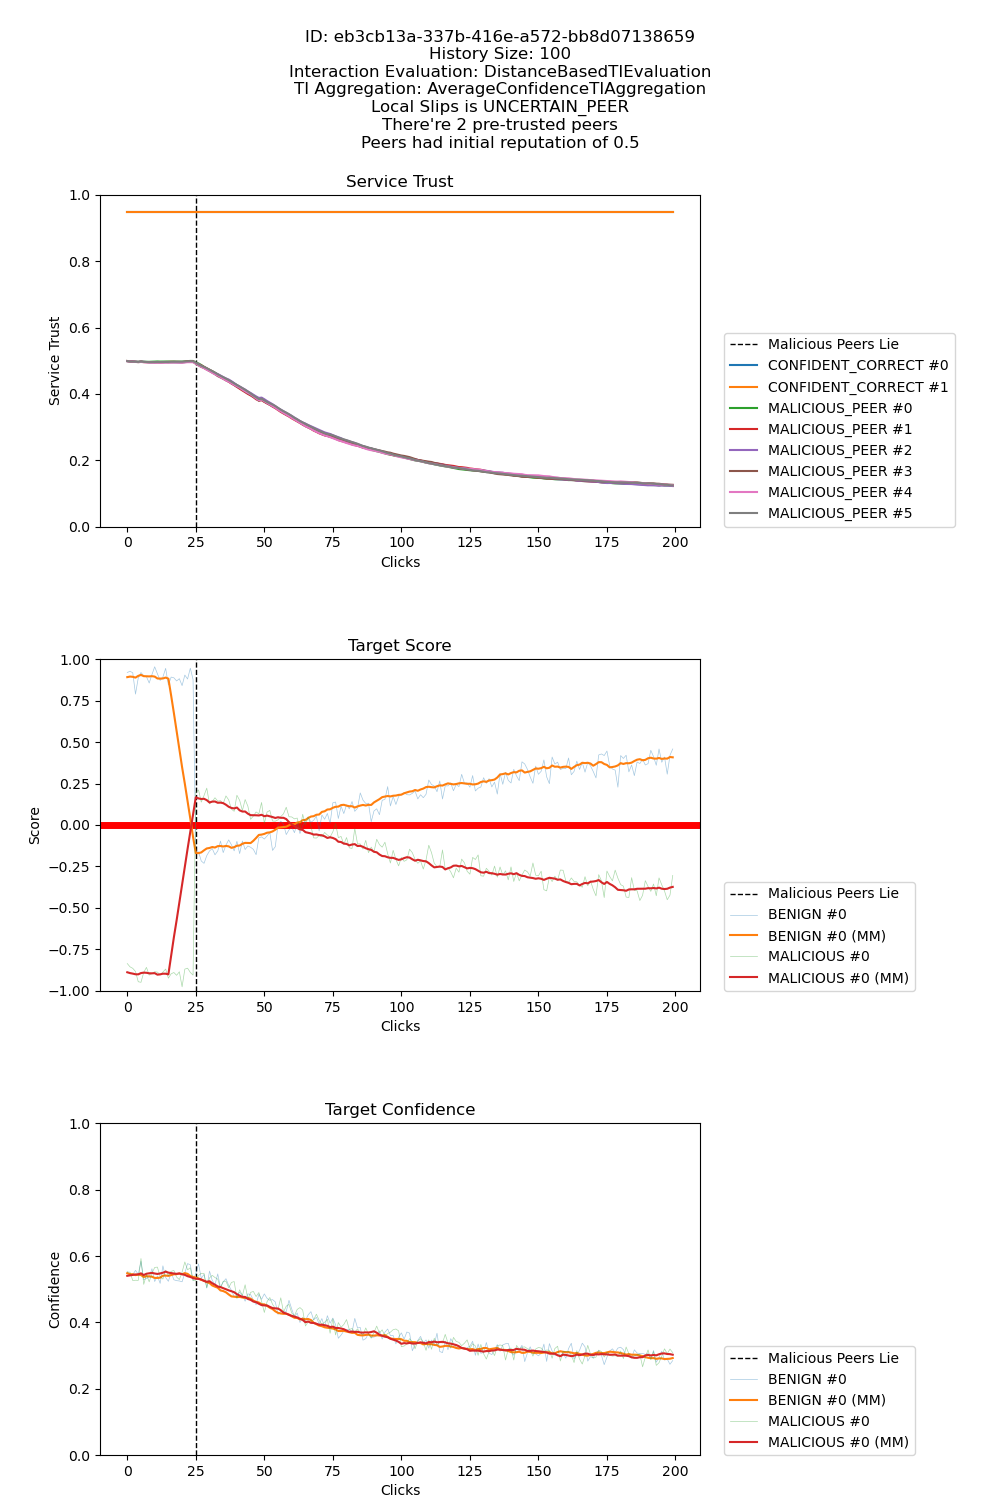
\includegraphics[width=1.0\textwidth]{assets/miss_classification_recovery.png}
    \caption{A scenario described in section \ref{subsec:correct-target-identification-no-matter-what} with initial reputation 0.5}
    \label{fig:missclassification-recovery}
\end{figure}

\begin{figure}
    \centering
    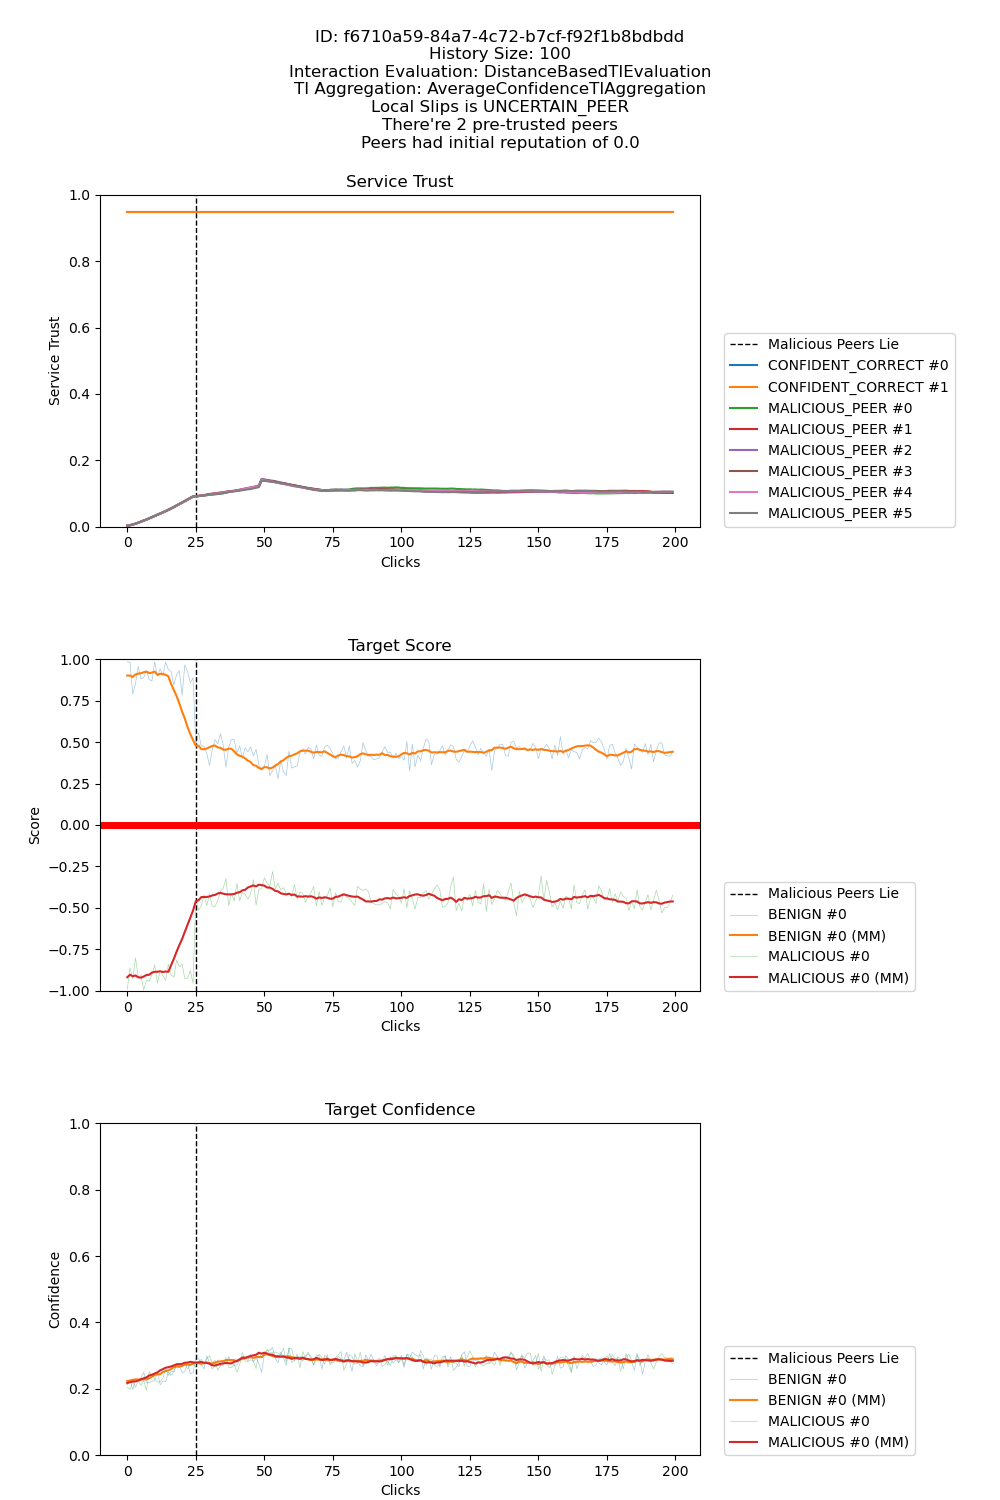
\includegraphics[width=1.0\textwidth]{assets/best_worst_case}
    \caption{A scenario described in section \ref{subsec:correct-target-identification-no-matter-what} with initial reputation 0}
    \label{fig:worst-best-scenario}
\end{figure}

\begin{figure}
    \centering
    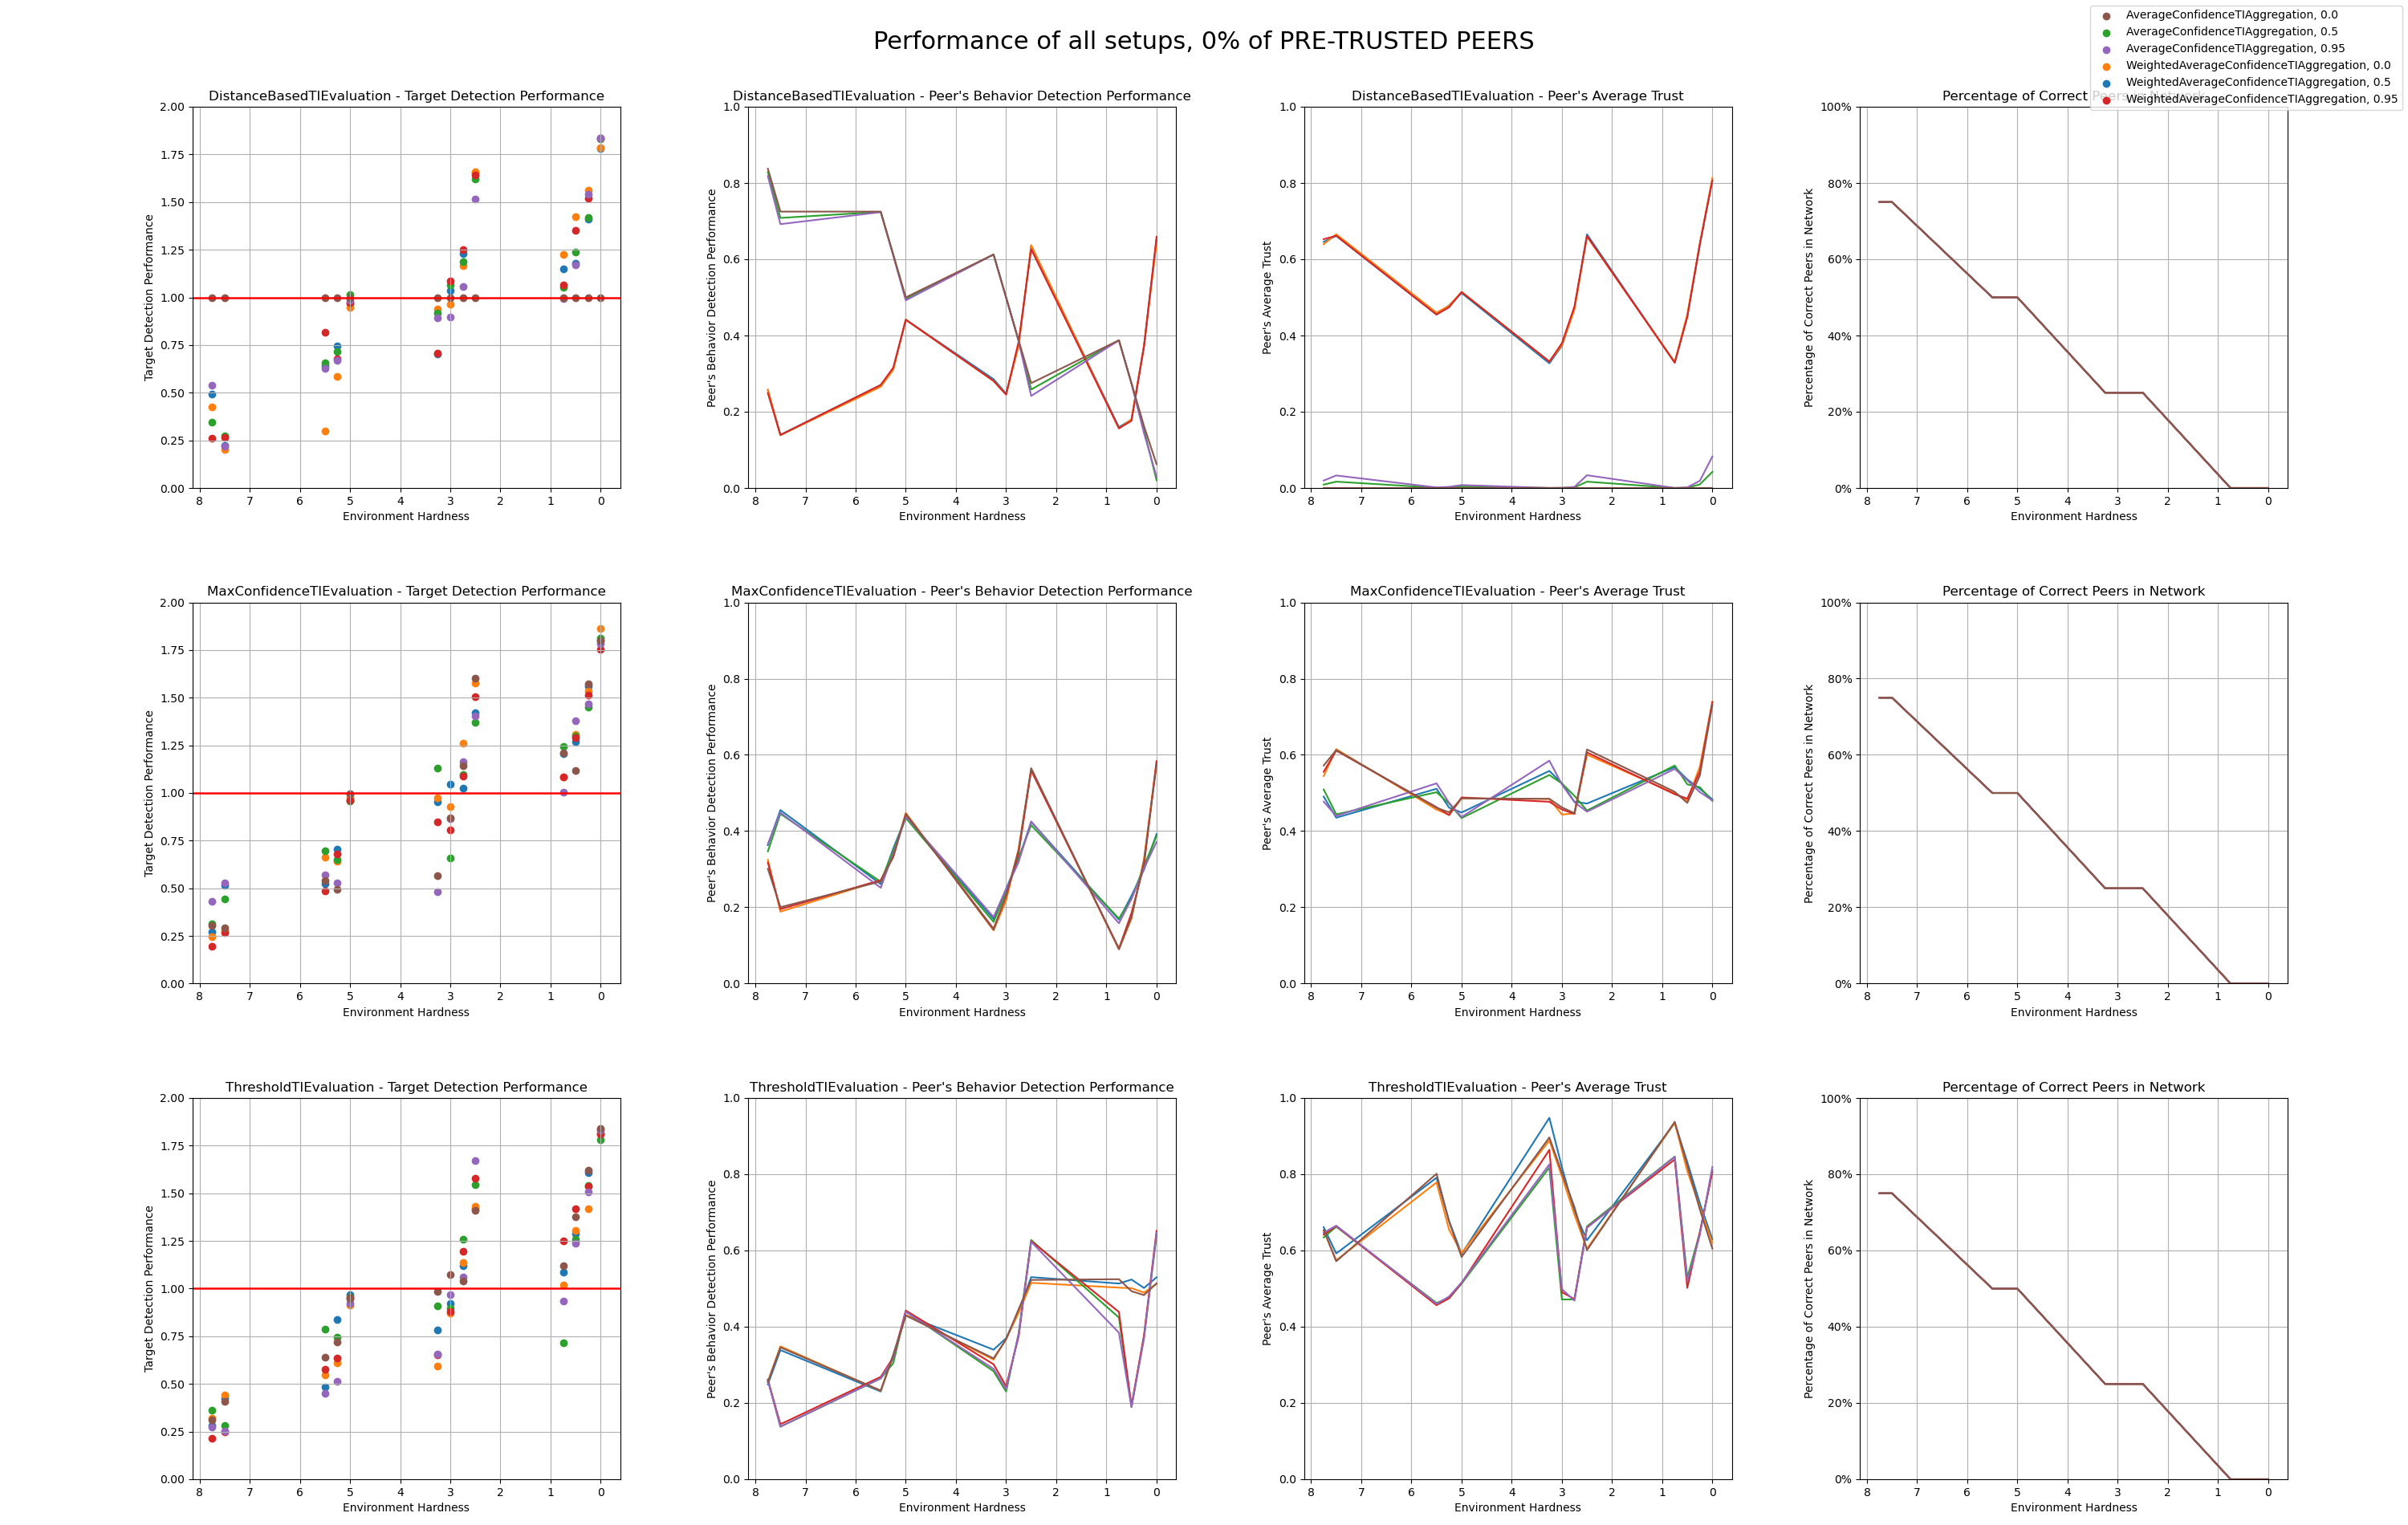
\includegraphics[width=0.9\paperwidth, angle=90]{assets/0_all_metrics.png}
    \caption{Evaluation of performance of all trust model setups with no pre-trusted peers}
    \label{fig:performance-all-setups-0-pretrusted}
\end{figure}

\begin{figure}
    \centering
    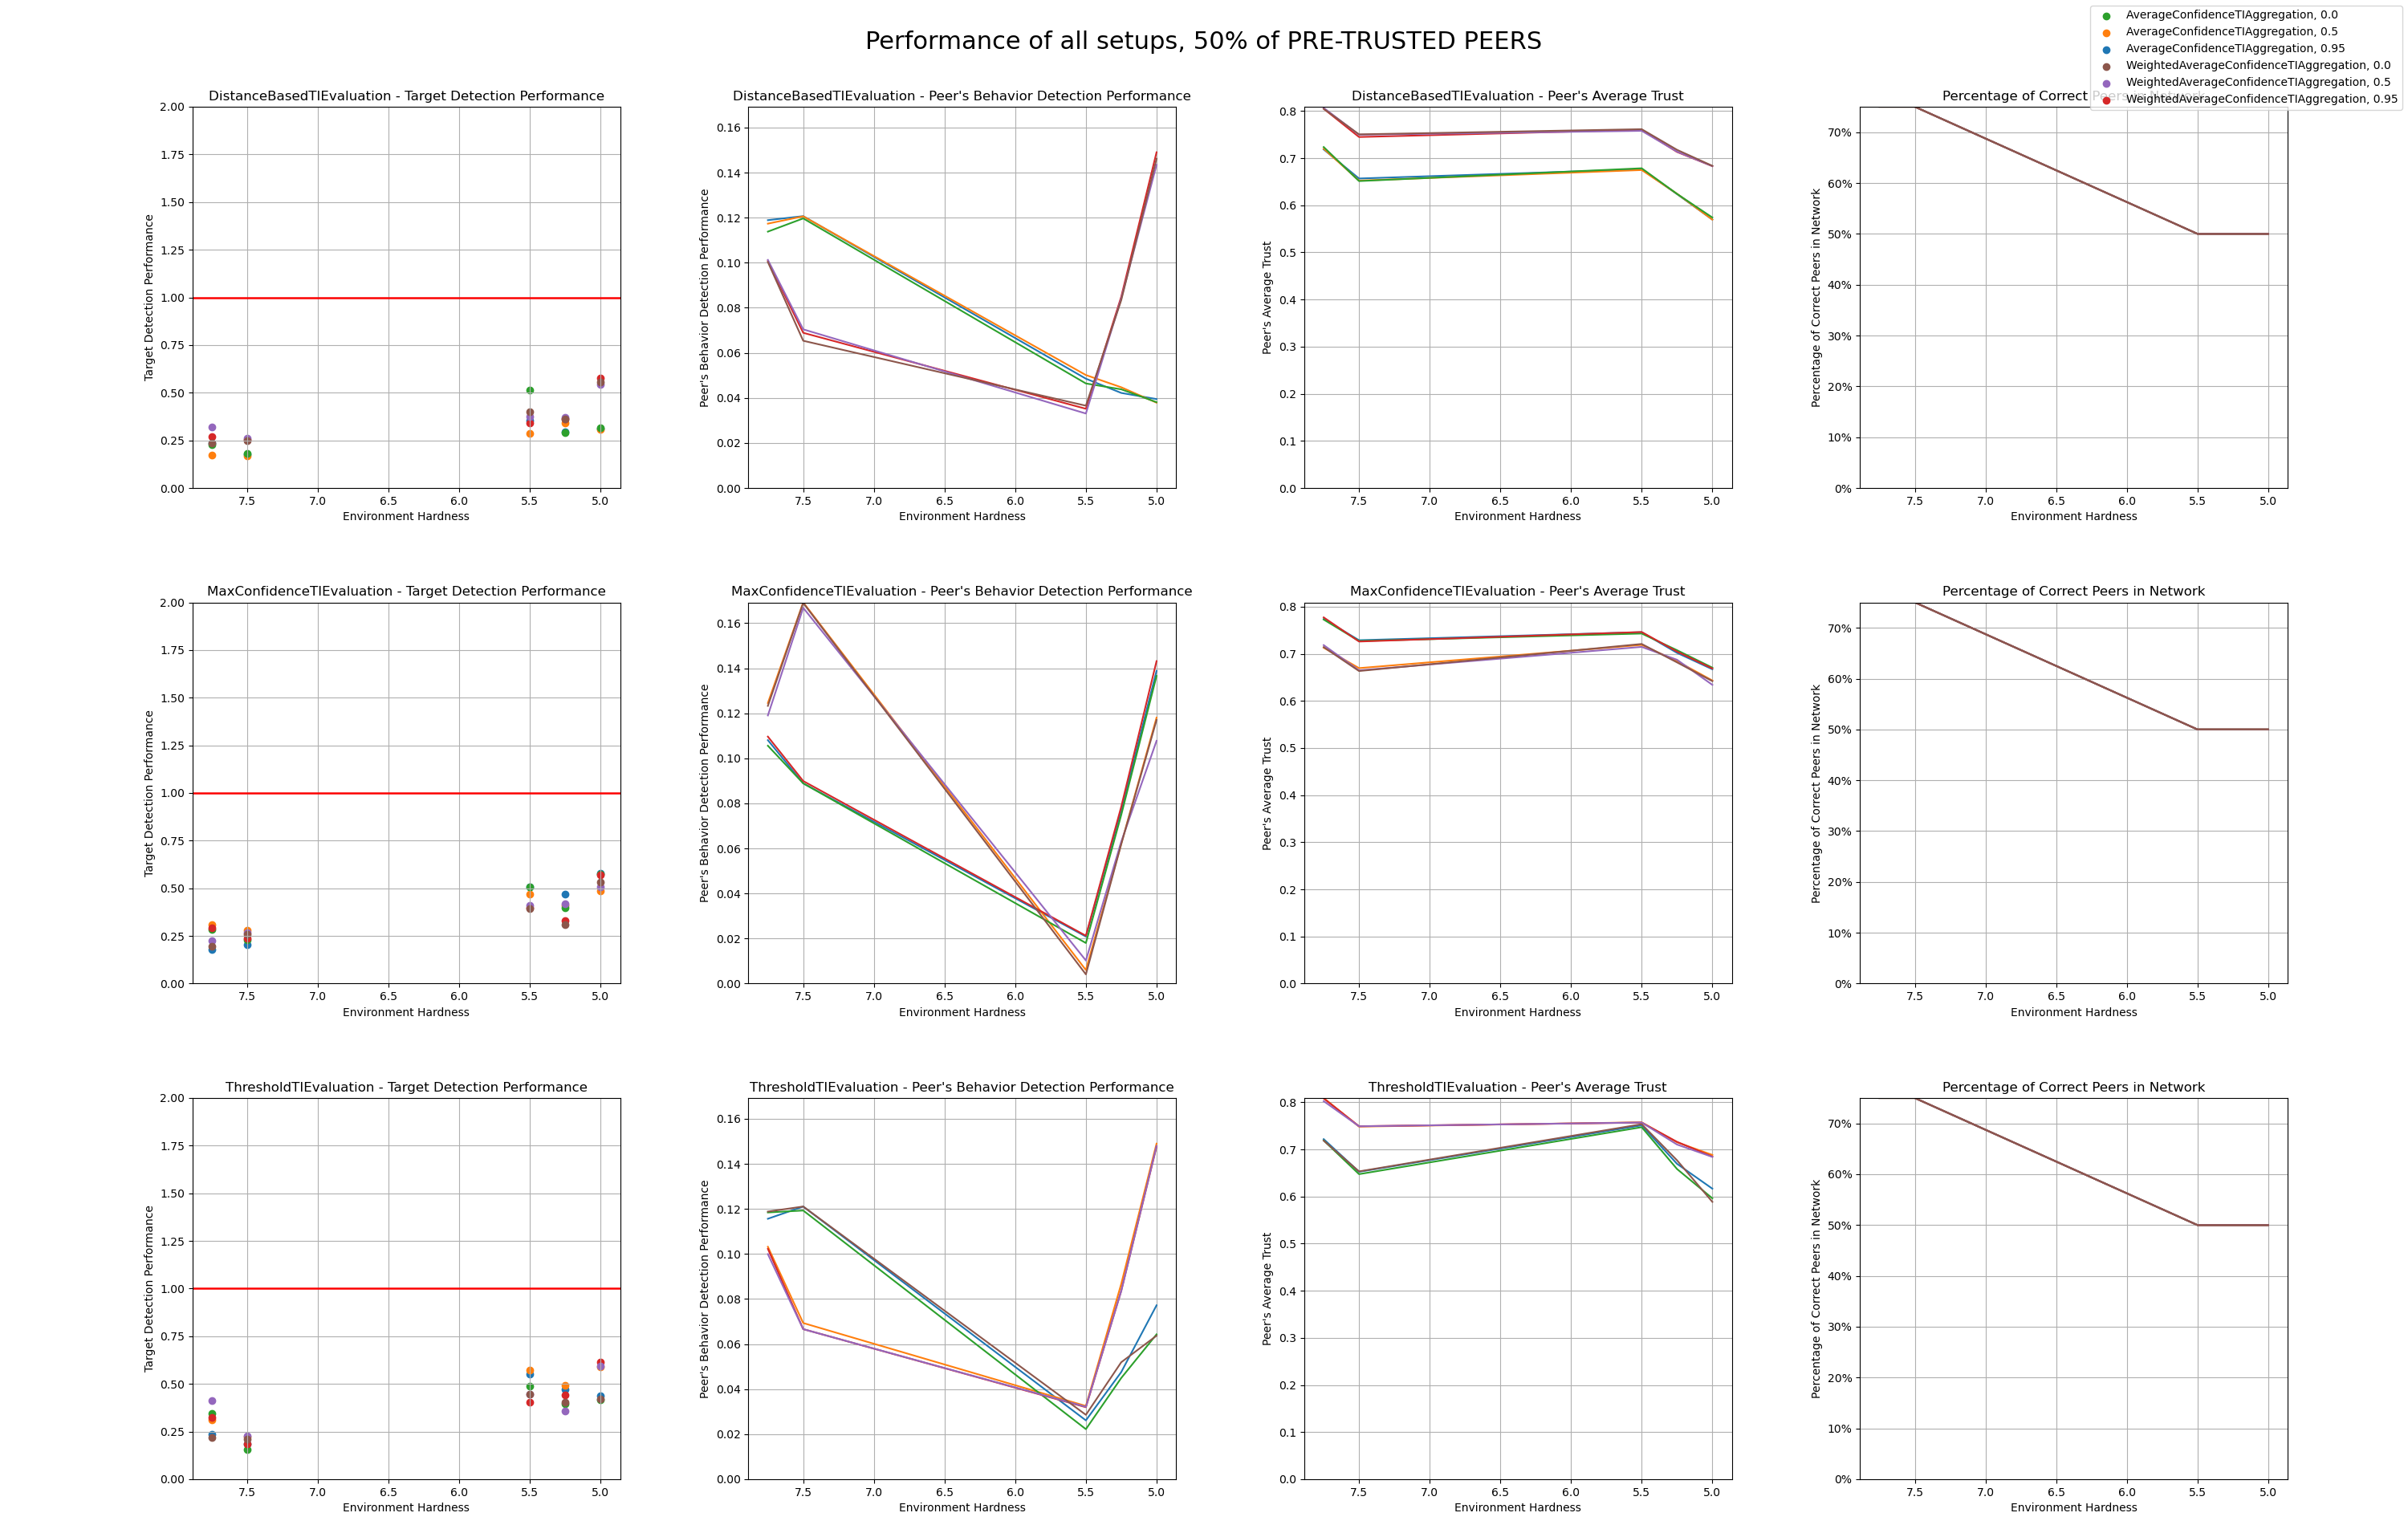
\includegraphics[width=0.9\paperwidth, angle=90]{assets/50_all_metrics.png}
    \caption{Evaluation of performance of all trust model setups with 50\% of pre-trusted peers}
    \label{fig:performance-all-setups-50-pretrusted}
\end{figure}

\begin{figure}
    \centering
    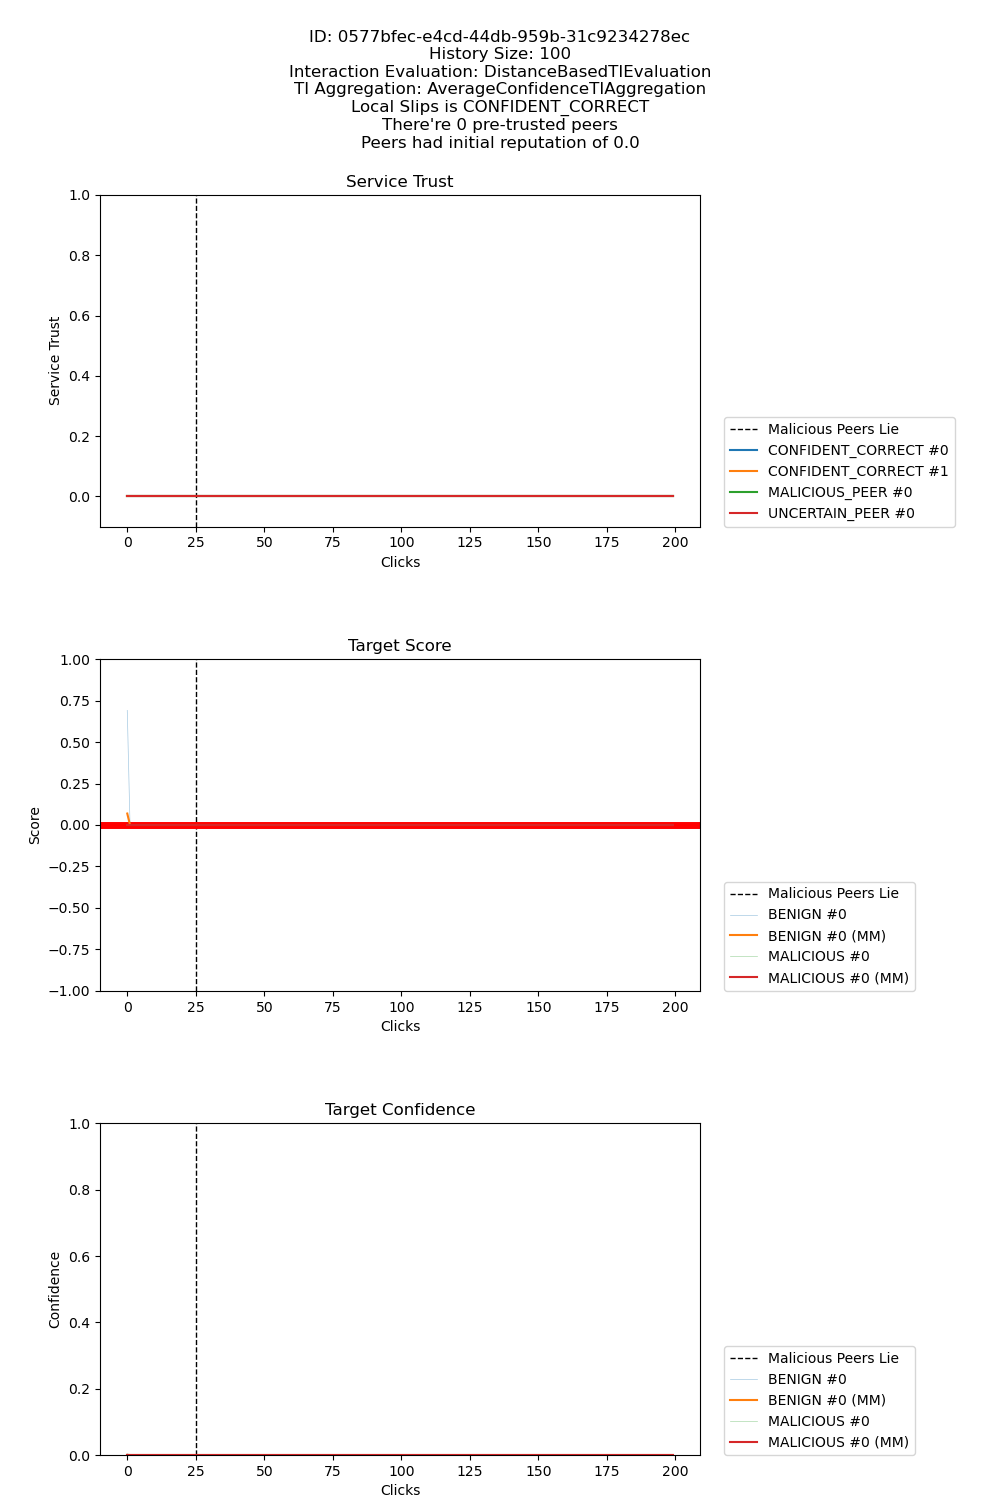
\includegraphics[width=1.0\textwidth]{assets/zero_gained_trust_all.png}
    \caption{Complete graph with all metrics from \ref{fig:zero-gained-trust}}
    \label{fig:zero-gained-trust-all}
\end{figure}

\newpage
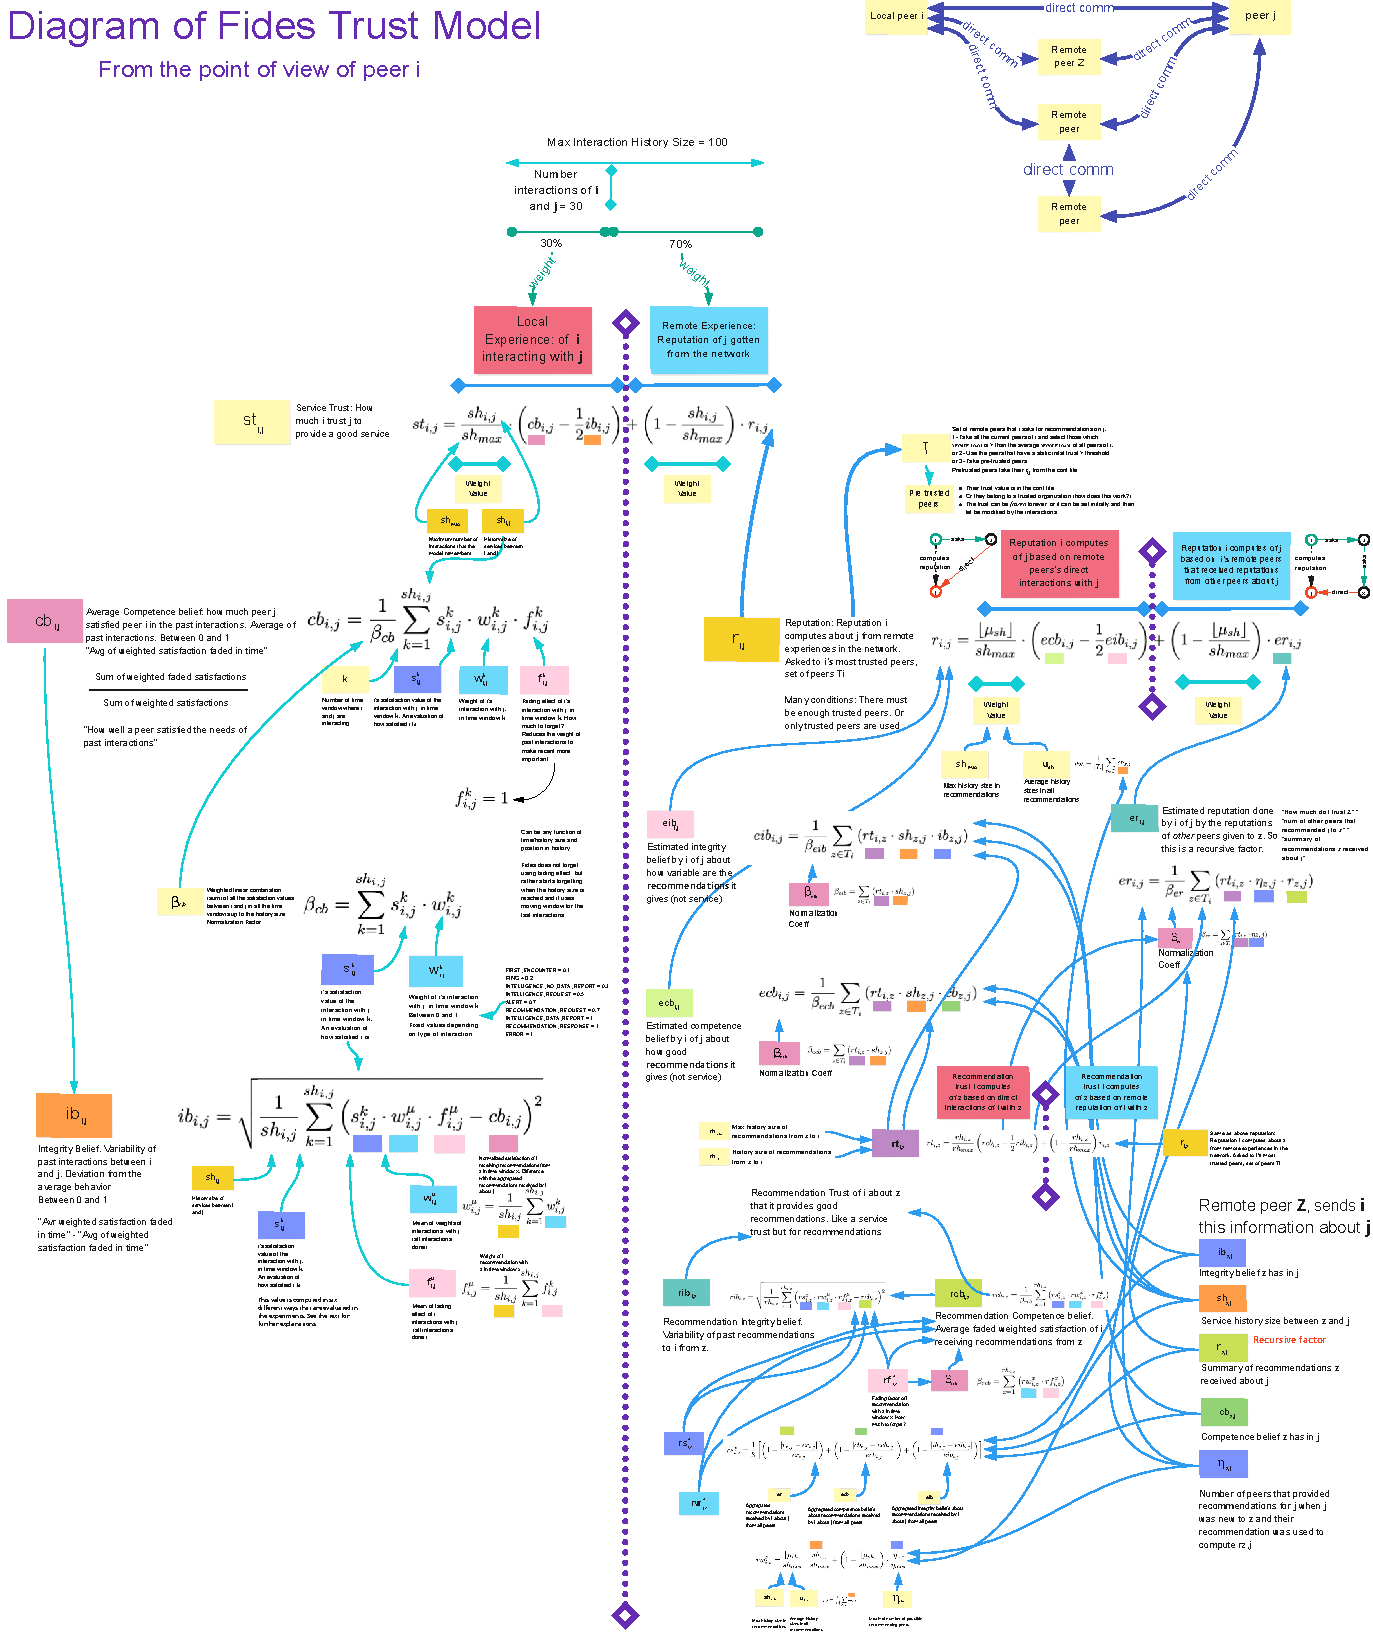
\includepdf[pages=-,scale=0.8]{assets/trust_model_scheme.pdf}

\end{document}
